\documentclass[11pt]{article}

\usepackage[T1]{fontenc}
\usepackage[utf8]{inputenc}
\usepackage{newtxtext,newtxmath}
\usepackage[margin=1in]{geometry}
\usepackage{microtype}
\usepackage{amsmath}
\usepackage{booktabs}
\usepackage{multirow}
\usepackage{threeparttable}
\usepackage{xcolor}
\usepackage{graphicx}
\usepackage{caption}
\usepackage{subcaption}
\usepackage{enumitem}
\usepackage{listings}
\usepackage[section]{placeins}
\usepackage{pgfplots}
\pgfplotsset{compat=1.18}
\usepackage[numbers,sort&compress]{natbib}
\usepackage[hidelinks]{hyperref}
\usepackage[capitalise,noabbrev]{cleveref}

\definecolor{ink}{HTML}{1F2328}
\definecolor{muted}{HTML}{6A737D}
\definecolor{kube}{HTML}{326CE5}
\definecolor{flyte}{HTML}{8A4FD3}
\definecolor{codebg}{HTML}{F6F8FA}

\lstdefinestyle{code}{
  basicstyle=\ttfamily\scriptsize,
  backgroundcolor=\color{codebg},
  frame=single, rulecolor=\color{codebg},
  columns=fullflexible, keepspaces=true,
  breaklines=true, breakatwhitespace=false,
  showstringspaces=false,
  xleftmargin=2pt, xrightmargin=2pt,
}
\lstset{style=code}

\renewcommand{\topfraction}{0.9}
\renewcommand{\bottomfraction}{0.8}
\renewcommand{\textfraction}{0.07}
\renewcommand{\floatpagefraction}{0.7}
\setcounter{topnumber}{3}
\setcounter{totalnumber}{5}
\captionsetup{font=small,labelfont=bf}
\setlist{nosep,leftmargin=*}
\newcommand{\code}[1]{\texttt{#1}}
\newcommand{\pp}{\,pp}
\newcommand{\ci}[2]{\,[#1,\,#2]}

\title{RightSize Bench: Learning Kubernetes Resource Requests from Code\\[2pt]
\large Sizing the pod before it runs, through a raw Job or an AI-native interface}
\author{Niels Bantilan\\ Union.ai\\ \texttt{niels@union.ai}}
\date{November 2026}

\begin{document}
\maketitle

\begin{abstract}
Before a batch pod runs on Kubernetes, someone has to decide how much memory and CPU it gets and whether
it gets a GPU. Too little makes it fail or run slowly, and too much wastes the cluster. We present
RightSize Bench, a benchmark that scores this decision in dollars: each request is replayed against a
measured run, failed attempts and throttling included, and compared with the cheapest request that would
have run it. The benchmark has 32,082 measured runs of 33 families of generated Python tasks that use real
libraries, from dataframes and SQL to PyTorch training and sharded language models. Every run appears
twice, as a raw Kubernetes Job whose inputs are staged in one of four ways, and as a task submitted
through Flyte, an orchestrator whose runtime we measure at about 70\,MiB per pod. We checked the Job labels
in about 480 real pods, which found two errors in our first release.

We release the benchmark with a set of baseline models: gradient-boosted quantile trees, and a 1.7B
decision model whose pointer heads score the request options written in its prompt, trained with
cross-entropy and then with reinforcement learning against the cost. On new tasks from familiar families,
the trees pooled with the decision model come within \rTestPoolDec\% of the cheapest request on Job pods,
against \rTestSized\% for a rule that scales earlier runs by input size and reads the pod spec, and
\rTestZS\% for a zero-shot 27B model. On seven held-out families every approach does much worse, and the
rule (\rUnseenSized\%) is as good as anything we trained. Models trained on Jobs move their memory request
with the volume medium in the manifest about three times in four. \codeSeenShare\% of the test tasks share
their exact code with a training task, so the held-out families are the benchmark's test of new code.
\end{abstract}

\section{Introduction}
\label{sec:intro}

Every container that runs on Kubernetes asks for resources before it starts~\citep{k8sresources}.
The numbers matter in different ways. Memory is a hard limit, so a container that
uses more than it asked for is killed and has to be run again. CPU is a soft limit, so a
container that wants more cores than it was given is throttled and finishes late. A GPU
is a choice of machine: if it is too small the task runs out of device memory, if it is
missing a GPU task fails at start, and if a CPU task gets one it pays for hardware it
never uses. In practice engineers pick these numbers by hand, usually once and usually
generously, and large clusters run well below what their jobs
reserve~\citep{verma2015borg,tirmazi2020borg}.

Autoscalers that learn from usage history~\citep{rzadca2020autopilot,k8svpa} work well for
long-running services. Batch work is harder. The first run of a batch task has no
history, and later runs often see inputs of a different size. Still, much of what
decides the right request is known before the pod starts. A scheduler can read the code
the pod will run, the size and format of its inputs, the way the pod spec stages those
inputs, and what earlier runs of the same task used. This paper asks how well different
approaches turn that information into a request, and measures the answer in dollars.

We treat the Kubernetes pod as the unit of work throughout. Teams submit pods in
different ways. The most direct is a \code{batch/v1} Job, which pairs a container image
with a manifest. Another is to write a typed Python function and let an orchestrator
build the pod. We use Flyte~\citep{flyte} as the example of the second route. Flyte acts
as an AI-native interface to Kubernetes: it turns a function into a pod, and adds typed
inputs and outputs, caching, retries and durable execution along the way. In both cases
the same user code runs in the same kind of pod. The differences are at the edges of the
pod, in how inputs arrive, what else shares the container, and what the monitoring
history reports. For Flyte, those conveniences cost 55--70\,MiB of runtime memory in the
task's container, which we measure directly (\cref{sec:validation}).

This paper makes five contributions.
\begin{enumerate}
  \item We build a benchmark of the whole pod request from 32,082 measured runs of 33
  families of generated Python tasks, covering dataframes, SQL, linear algebra,
  classical ML, PyTorch training and inference, and sharded language models. Each run
  has measured peak memory, CPU use at the 15-second resolution of cluster monitoring,
  and peak GPU memory across seven machine shapes (\cref{sec:dataset}).
  \item We present every run both as a raw Kubernetes Job and as a Flyte task. The Job
  stages its inputs in one of four ways, and its labels follow from an explicit
  accounting of what differs between the two pods (\cref{sec:twins}).
  \item We check that accounting in about 480 real pods, reading each container's own
  cgroup counters (\cref{sec:validation}). The check found two defects in our first
  release, both now fixed. The Flyte runtime constant was 2.6 times too large, and some
  init containers were too small to hold the inputs they staged. It also showed that the
  standard \code{ru\_maxrss} measurement leaves about a third of labels one cell higher
  than necessary.
  \item We score requests with a single cost model that covers memory, CPU and GPU
  together, and report both mean and dollar-weighted regret with task-clustered
  confidence intervals (\cref{sec:cost}).
  \item We compare eleven kinds of approach over three independent trainings, from static
  requests and hand-written rules to gradient-boosted trees, a zero-shot 27B model, a
  fine-tuned 1.7B decision model trained further with reinforcement learning, opinion
  pools, and a pre-registered novelty gate (\cref{sec:methods,sec:results}). Two
  controlled tests ask what the models actually read. One changes only the manifest, and
  the other removes the task's name from its code.
\end{enumerate}

\section{Background: one pod, two ways to submit it}
\label{sec:background}

\paragraph{Requests, limits and cgroups.}
Each Kubernetes container declares a memory and CPU \emph{request}, which the scheduler
reserves on a node, and a \emph{limit}, which the kubelet enforces through the
container's cgroup~\citep{k8sresources,cgroupv2}. Under cgroup~v2, a container whose
charged memory reaches its limit is OOM-killed. Both anonymous memory and shared memory
(\code{shmem}) count toward that limit, while clean page cache does not, because the
kernel can reclaim it first. A CPU limit works differently. It is enforced as a CFS
quota, so a container that exceeds it is slowed down rather than killed. Accelerators are
requested as whole devices on node pools that carry them. In this paper a request also
sets the limit, which is the usual choice for batch pods because it makes scheduling and
failures predictable.

\paragraph{How the pod spec changes a task's memory.}
Three details of a pod spec can change how much memory a batch task needs without any
change to its code. The first is the medium of the volume that holds its inputs. An
\code{emptyDir} on node disk keeps files as page cache, which the kernel reclaims under
pressure. An \code{emptyDir} with \code{medium: Memory} is a tmpfs, and every byte written
to it is charged to memory as \code{shmem}~\citep{k8svolumes}. Staging a 2\,GiB input on
tmpfs therefore adds 2\,GiB to the pod's need. The second detail is who fetches the
inputs. An init container runs to completion before the main container starts and has
its own limit, whereas a download inside the job runs in the job's container, so the
client library's memory and threads count against the job. The third is anything else
that shares the container, such as an orchestration runtime or a client library.

There is one subtlety with tmpfs. A page is charged to the cgroup of the container that
writes it, so pages written by an init container are not charged to the main container.
When the init container exits, though, its pages move to the pod's cgroup and still count
against the pod's overall limit. We confirm this in real pods in
\cref{sec:validation}.

\paragraph{Raw Jobs.}
A \code{batch/v1} Job runs a pod template until it succeeds. Its \code{backoffLimit}
says how many failed pods it will replace before giving up. Batch teams often set it to
zero and resubmit failures by hand or from an outer scheduler. A Job has to stage its own
inputs, either with an init container or in the job's code.

\paragraph{Flyte as an interface to Kubernetes.}
Flyte~\citep{flyte} turns a typed Python function into a Kubernetes pod. A user writes
\code{@env.task async def f(x: File) -> dict}, and Flyte builds the image, renders the
pod spec, moves typed inputs and outputs through object storage, caches results by their
inputs, retries failed attempts, and records each execution so that a long pipeline can
resume after a node is lost. None of this changes what the function does inside the
container. It changes the pod's edges instead. Inputs arrive through Flyte's own
download, the container also runs Flyte's runtime, and the execution history reports the
container's peak with that runtime included. We measure the runtime at 55\,MiB at rest,
and a median 70\,MiB above the same workload run as a plain Job (\cref{sec:validation}).

For resource sizing, then, Flyte is a convenience layer over the same pod. It costs a
little memory in exchange for typed I/O, caching, retries and durable execution. An
approach that can size a Kubernetes pod should be able to size a Flyte task using the
same knowledge plus the runtime.

\section{Related work}
\label{sec:related}

\paragraph{Sizing from history.}
Autopilot~\citep{rzadca2020autopilot} sets Google's container limits from the usage
history of a job's tasks, using moving-window and ML recommenders. Kubernetes' Vertical
Pod Autoscaler~\citep{k8svpa} recommends requests from a decaying histogram of observed
usage. Borg traces show that most jobs over-request~\citep{verma2015borg,tirmazi2020borg}.
Resource Central~\citep{cortez2017resourcecentral} predicts VM utilization from a
subscription's history. All of these size workloads that have run before, and run long
enough to observe. RightSize Bench reports first runs (no history) and runs with history
separately. Quasar~\citep{delimitrou2014quasar} classifies new workloads from short
profiling runs; RightSize Bench allows no profiling, only what a scheduler can read
before the pod starts.

\paragraph{Learned predictors.}
Quantile regression~\citep{koenker1978quantile} with gradient-boosted
trees~\citep{friedman2001gbm,ke2017lightgbm} is a standard way to predict a distribution
of resource need; it is the strongest classical approach here. Our decision model
replaces a language model's output layer with a pointer head~\citep{vinyals2015pointer}
that scores option tokens written in the prompt. It is adapted with LoRA~\citep{hu2022lora}
on Qwen3~\citep{qwen3}.

\paragraph{Training on the objective.}
Group-relative policy optimization (GRPO)~\citep{shao2024deepseekmath} drops PPO's value
network by normalizing rewards within a group of samples for the same prompt. We use that
group-normalized advantage with a single on-policy step per batch. Our policy is three
categorical distributions, so a group is sampled from one forward pass, and the reward is the
benchmark's own cost simulator.

\paragraph{Combining and routing models.}
Logarithmic opinion pools~\citep{genest1986pools} combine calibrated distributions by a
weighted geometric mean. Temperature scaling~\citep{guo2017calibration} calibrates each
model before pooling. Distance to the $k$ nearest training points is a common
out-of-distribution signal~\citep{sun2022knnood}; our gate uses it to choose between two
models.

\section{Problem}
\label{sec:problem}

A \emph{run} is one execution of a task on one set of inputs, in one pod. Before the pod starts, an approach
may look at three things. The first is the task's code as it was submitted: \code{job.py} and the Job manifest
for a raw Job, and the task module for a Flyte task (\cref{sec:twins}). The second is the metadata a scheduler
can read about this run's inputs: their sizes and formats and whatever the format's header exposes, such as
the row count and schema of a Parquet file or the shape and dtype of a \code{.npy} array. The third is what
earlier runs of the same task used: their peak memory, peak and mean cores, peak GPU memory and utilization,
wall time and input sizes. These are reported the way the platform's monitoring would show them, which means
the container's own peak for a Job and the peak including the runtime for a Flyte task.

An approach is never given the task's family, the hidden settings it was generated with, the corpus it came
from, or anything measured on the run itself. A unit test checks that changing those fields leaves the
features and the prompt unchanged. The code does identify the family in practice: each task is named after its
family, and each family's generator has a fixed function name and input schema. \Cref{sec:res-manifest}
re-scores with neutral names.

From what it can see, the approach chooses a request on three axes (\cref{tab:grid}). A GPU request lands on
the cheapest machine that can hold it (\cref{tab:ladder}). On a GPU node the host memory and cores come with
the instance, so they are not scored.

\begin{table}[tbp]
\centering\small
\caption{The request grid.}
\label{tab:grid}
\begin{tabular}{@{}lrl@{}}
\toprule
axis & cells & values \\
\midrule
memory & 17 & 256, 384, 512, 768\,Mi; 1, 1.5, 2, 3, 4, 6, 8, 12, 16, 24, 32, 48, 64\,Gi (half powers of two) \\
CPU    & 16 & 0.25, 0.5, 0.75, 1, 1.25, 1.5, 1.75, 2, 2.5, 3, 3.5, 4, 5, 6, 7, 8 cores \\
GPU    & 18 & none, or peak GPU memory 1, 1.5, 2, 3, 4, 6, 8, 10, 12, 15, 22, 32, 44, 64, 88, 120, 176\,GiB \\
\bottomrule
\end{tabular}
\end{table}

\begin{table}[tbp]
\centering\small
\caption{The GPU machine ladder: the cluster's GPU node pools, with on-demand \code{us-east-1} prices for the
whole node. Usable GiB is NVML's total, rounded down. The A10G is never the cheapest shape for any cell.}
\label{tab:ladder}
\begin{tabular}{@{}llrrr@{}}
\toprule
shape & instance & GPUs & usable GiB & \$/h \\
\midrule
T4      & g4dn.xlarge  & 1 & 15         & 0.526 \\
L4      & g6.2xlarge   & 1 & 22         & 0.978 \\
A10G    & g5.2xlarge   & 1 & 22         & 1.212 \\
L40S    & g6e.2xlarge  & 1 & 44         & 2.242 \\
4$\times$L4   & g6.12xlarge  & 4 & 4$\times$22 & 4.602 \\
8$\times$T4   & g4dn.metal   & 8 & 8$\times$15 & 7.824 \\
4$\times$L40S & g6e.12xlarge & 4 & 4$\times$44 & 10.493 \\
\bottomrule
\end{tabular}
\end{table}

\section{Dataset}
\label{sec:dataset}

The benchmark combines three corpora. Each one was built by its own single-axis benchmark
using the same recipe. We wrote families of code generators, sampled tasks from each
family, and measured several runs of each task at different input sizes in Kubernetes
pods. \Cref{tab:corpora} summarizes the three corpora, and \cref{app:families} lists every
family. All of these measurements describe the workload itself, independent of how its
pod was submitted. \Cref{sec:twins} then works out what a Job pod and a Flyte pod each
need, starting from the same measurement.

\begin{table}[tbp]
\centering\small
\caption{The three corpora. RightSizeGPU's 2,052 unusable runs: 1,569 censored (out of
memory on the largest shape they reached), 51 failed, and 432 the combined bench drops
because their peak filled the device, which makes the measured peak only a lower bound.
RightSizeMem's 166 unusable runs exceeded its 20\,GiB guard or 900\,s timeout.}
\label{tab:corpora}
\resizebox{\linewidth}{!}{%
\begin{tabular}{@{}llrrrrrrl@{}}
\toprule
corpus & release & families & held out & tasks/fam. & runs/task & measured & usable & labels \\
\midrule
RightSizeMem & v2    & 12 & 2 & 400 & 3 & 14,400 & 14,234 & peak memory; mean cores \\
RightSizeCPU & big-1 & 11 & 2 & 450 & 2 &  9,900 &  9,900 & peak memory; busiest 15\,s \\
RightSizeGPU & big-2 & 10 & 3 & 500 & 2 & 10,000 &  7,948 & peak GPU memory, sharding \\
\midrule
combined     & k8s-2 & 33 & 7 &     &   & 34,300 & 32,082 & \\
\bottomrule
\end{tabular}}
\end{table}

\subsection{Families, tasks and runs}
A \emph{family} is a Python generator. Given a seed, it writes a task function and the
specification of its inputs, and it draws a few hidden settings, which we call knobs,
that decide how input bytes turn into resource use. A pandas family, for example,
decides whether to project columns, which dtype backend to use and whether to downcast
floats. A training family picks width, depth, batch size, mixed precision and
checkpointing, and a CPU family picks a thread-pool size or leaves it unset. The knobs
show up only in the code an approach reads. They are never given to an approach directly,
and we keep them only to slice the results.

Each run scales the leading dimension of the task's inputs by a factor drawn
log-uniformly from $[0.25, 4]$ for RightSizeMem and from $[0.5, 2]$ for the CPU and GPU
corpora. Runs are shuffled, so a task's history can be larger or smaller than the current
run. The inputs are synthetic: normal floats, uniform integers, dictionary-encoded
categories, random strings, Zipf-distributed word ids for text, and random bytes for
images, written as Parquet, CSV, JSONL or \code{.npy}. CPU and GPU workloads loop until a
per-task time budget runs out (30--60\,s for CPU and 45--90\,s for GPU), while RightSizeMem
workloads run to completion.

\subsection{RightSizeMem v2: peak memory}
RightSizeMem has twelve families, chosen because they turn input bytes into memory in
different ways. They include pandas group-bys and joins, polars pipelines in eager, lazy
and streaming modes, DuckDB queries with and without a memory limit, chunked CSV and
JSONL readers, NumPy linear algebra with optional memory mapping, scikit-learn
estimators, TF-IDF, a small PyTorch model on CPU, image batches and pure-Python grouping.

Each run uses three processes. A child process writes the inputs to a temporary
directory, a fresh interpreter runs the task body on those files, and the parent reads
the child's \code{ru\_maxrss} and CPU time from \code{wait4}. BLAS and OpenMP are limited
to one thread, and workloads set their own threads in code. The workload's peak memory
$w$ is its \code{ru\_maxrss}. As we show in \cref{sec:validation}, on Linux this value
includes the measuring parent's own peak at the time of \code{exec}, about 158\,MiB here,
which makes about a third of the smaller workloads' labels one cell higher than needed.

\subsection{RightSizeCPU big-1: the busiest 15 seconds}
RightSizeCPU has eleven families, chosen for how they use cores, since CPU need depends on
parallelism much more than on input size. They cover NumPy BLAS with and without a thread
cap, polars and DuckDB with explicit thread settings, scikit-learn ensembles, serial
pandas, Python thread pools that hold or release the GIL, process pools, a CPU PyTorch
model, pyarrow CSV parsing, an I/O-bound pool and a task with two phases.

CPU time for the whole process tree is sampled every second. Each pod runs two
measurements side by side on disjoint sets of seven cores, and a check of 44 runs
against single-run pods put all 44 within 25\% of each other. The CPU label is the
busiest 15-second average, because that is the resolution at which cluster monitoring
(Prometheus scraping cAdvisor every 15\,s) sees a container. Peak memory is measured as in
RightSizeMem.

\subsection{RightSizeGPU big-2: peak GPU memory across a machine ladder}
RightSizeGPU has ten PyTorch families: a tabular MLP, a CNN, a CNN limited by its data
loader, a GPT language model, a transformer encoder, a recommender with sharded
embeddings, blocked matrix multiplication, nearest-neighbour search, fine-tuning of
decoders from 0.6B to 7B parameters split across GPUs, and generation with a KV cache.
NVML reports memory and utilization on every visible GPU every half second. Each run
starts on a T4 and moves up the machine ladder (\cref{tab:ladder}) whenever it runs out
of device memory, and a run that runs out of memory on the largest machine it reached is
censored. The oracle machine for a run is the cheapest one it fits on. For machines a run
was not measured on, we model the fit from its per-GPU peak and, for sharded code, its
imbalance across GPUs.

\subsection{Splits and history}
Runs are split by task, never by run. A hash of the task id sends 70\% of each family's
tasks to training, 10\% to validation and 20\% to test. The seven held-out families go
entirely to a separate \emph{unseen} split. The test split therefore measures how well an
approach handles new tasks from familiar families, and the unseen split measures how well
it handles new kinds of code. Every setting that an approach tunes is chosen on
validation, which contains familiar families only.

The $k$-th run of a task carries the task's earlier runs as its history. A task's first
run has no history at all, and these cold starts make up 33--50\% of each split.

\begin{table}[tbp]
\centering\small
\caption{Usable runs per split. Each run appears twice in the bench, once as a Job and
once as a Flyte task, in the same split.}
\label{tab:splits}
\begin{tabular}{@{}lrrrrl@{}}
\toprule
source & train & val & test & unseen & unseen families \\
\midrule
mem & 8,457 & 1,138 & 2,316 & 2,323 & duckdb\_sql, image\_batch \\
cpu & 5,628 &   838 & 1,634 & 1,800 & duckdb\_sql, pyarrow\_csv \\
gpu & 3,968 &   542 & 1,145 & 2,293 & recsys\_train, knn\_search, llm\_generate \\
\midrule
runs        & 18,053 & 2,518 &  5,095 &  6,416 & \\
pods (rows) & 36,106 & 5,036 & 10,190 & 12,832 & \\
\bottomrule
\end{tabular}
\end{table}

\section{Every run as a Job and as a Flyte task}
\label{sec:twins}

The workload code was generated as Flyte tasks, but nothing in the body of a task
depends on Flyte. We use that to put every measured run into the benchmark twice, once as
a raw Kubernetes Job and once as a Flyte task, with the task body unchanged in both. To
make the Job version, \code{job.py}, we turn \code{File} parameters into paths, drop the
\code{flyte} import, and add a \code{\_\_main\_\_} block that stages the inputs, calls the
function and writes \code{result.json} for upload. A \code{batch/v1} manifest goes with
it, carrying the image, the input locations, the thread settings the measurement used,
the staging volume and an empty \code{resources} block, which is the request still to be
decided. \Cref{fig:twin} shows one task written both ways.

\begin{figure}[tbp]
\centering
\begin{minipage}[t]{0.48\linewidth}
\textbf{\small Flyte task}
\lstinputlisting[language=Python]{figures/ex_flyte.py}
\textbf{\small Job manifest (boto3-tmpfs)}
\lstinputlisting{figures/ex_manifest.yaml}
\end{minipage}\hfill
\begin{minipage}[t]{0.50\linewidth}
\textbf{\small \code{job.py} (boto3 staging)}
\lstinputlisting[language=Python]{figures/ex_job.py}
\end{minipage}
\caption{One RightSizeMem task, as a Flyte task and as a raw Job. The disk staging
differs from this manifest in one line, \code{emptyDir: \{\}}. The init-container
stagings add an \code{aws-cli} init container that copies the inputs to \code{/data}, and
\code{job.py} then reads them from \code{argv} (\cref{app:prompt}).}
\label{fig:twin}
\end{figure}

\subsection{Stagings}
How a Job's inputs reach its container is the biggest thing that changes its memory
need. Each task is assigned one of four stagings by a hash of its id, and all of its runs
share it (\cref{tab:stagings}). Inputs are fetched either by an init container running
\code{aws-cli} or by the job itself with boto3, and they land either on node disk or on a
memory-backed volume.

\begin{table}[tbp]
\centering\small
\caption{The four Job stagings.}
\label{tab:stagings}
\resizebox{\linewidth}{!}{%
\begin{tabular}{@{}lrlll@{}}
\toprule
staging & share & who fetches the inputs & where they land & memory need beyond the workload \\
\midrule
init-disk   & 30\% & aws-cli init container & \code{emptyDir} on node disk & --- \\
init-tmpfs  & 20\% & aws-cli init container & \code{emptyDir}, \code{medium: Memory} & $+B$ (staged bytes) \\
boto3-disk  & 30\% & the job itself, boto3  & \code{emptyDir} on node disk & $+48$\,MiB (boto3) \\
boto3-tmpfs & 20\% & the job itself, boto3  & \code{emptyDir}, \code{medium: Memory} & $+48$\,MiB $+B$ \\
\bottomrule
\end{tabular}}
\end{table}

\subsection{Label accounting}
\label{sec:accounting}
Let $w$ be the workload's measured peak memory (\cref{sec:dataset}) and let $B$ be the
size of the staged inputs plus the result file, with each file rounded up to whole pages.
The two kinds of pod need
\begin{align*}
\text{Job:}\quad & 1.05\,\bigl(w + 48\,\text{MiB}\cdot[\text{boto3}] + B\cdot[\text{tmpfs}]\bigr),\\
\text{Flyte:}\quad & 1.05\,\bigl(w + R\bigr), \qquad R = 70\,\text{MiB},
\end{align*}
where the factor 1.05 is headroom and the memory label is the smallest grid cell at or
above the need. Each term has a simple reason. Files on a memory-backed volume are
charged to memory byte for byte, while the same files on node disk are reclaimable page
cache and add nothing, since the measured workloads already read local files. The boto3
client adds 48\,MiB to a workload's peak. Its download also runs inside the job, taking
$d = \text{bytes}/440\,\text{MB/s} + 0.4\,\text{s per object} + 0.7\,\text{s}$ at about
1.8 cores, so we prepend that window to the run's CPU series. For a light job with a large
input, the download can be the busiest 15 seconds of the run. The Flyte runtime $R$ is
70\,MiB, measured in real task pods (\cref{sec:validation}). Earlier releases used a value
of 180\,MiB that had never been measured. Staging does not change GPU need.

The manifest sizes the init container at $256\,\text{MiB} + B$ for tmpfs stagings, so
that it can hold what it writes. Our first release used a flat 256\,Mi, which real pods
showed cannot work for larger inputs (\cref{sec:validation}). Histories are reported in
each interface's own units: a Job's earlier runs report the container's peak as cAdvisor
would, and a Flyte task's report the peak including the runtime, as Flyte's UI would.

The staging constants come from an in-cluster probe using boto3 1.43 under cgroup~v2. A
bare interpreter holds 11\,MiB. With boto3 imported, a client built and a file downloaded,
the process holds 74--80\,MiB, and it never peaks above that final level. Inside a real
workload boto3 adds only 48\,MiB at the median, because it shares modules the workload has
already loaded. Download throughput rises from 122\,MB/s for a 64\,MiB object to
417--431\,MB/s for a 4\,GiB one.

\section{Checking the labels in real pods}
\label{sec:validation}

The Job labels in \cref{sec:accounting} are derived from the workload's measurement, so we
checked them twice. The first check (rt-k8sval-2) re-ran 176 corpus runs both as Flyte
tasks and as their rendered \code{job.py}, as sibling processes inside one pod. It
confirmed the arithmetic of the accounting. Measured over predicted memory was
0.999--1.000 at the median for every staging, and tmpfs was charged at exactly the input
size. A pod with one container has one memory cgroup, so this check could not show
where the kernel charges pages when a pod has several containers.

The second check (rt-k8spod-1) used real pods. We took 100 runs (48 from RightSizeMem, 44
from RightSizeCPU, and 8 init-tmpfs runs with inputs over 300\,MiB) and gave each of them
pods of its own, about 480 in all (\cref{tab:podprobe}). Every container sampled its own
cgroup's memory counters every 50 milliseconds.

\begin{table}[tbp]
\centering\small
\caption{The pods in the real-pod check (rt-k8spod-1).}
\label{tab:podprobe}
\begin{tabular}{@{}lp{0.62\linewidth}@{}}
\toprule
pod & what it measures \\
\midrule
Flyte task & the run as a real Flyte task: the rendered module in a fresh task pod, with its inputs downloaded by Flyte \\
Job, generous limit & the pod the manifest describes, with each container reading its own cgroup \\
Job at its label & does the run fit when the job container's limit is set to the label? \\
Job one cell lower & does the cell below the label fail? \\
init-tmpfs extras & the first release's flat 256\,Mi init container, and the job at its label minus the staged bytes \\
\bottomrule
\end{tabular}
\end{table}

\paragraph{The Flyte runtime.}
Before a task's own module is imported, the Flyte task container already holds 55.0\,MiB
of anonymous memory, with almost no variation across the 100 runs (p10--p90
54.9--55.0\,MiB). Its peak is a median 70\,MiB above the same run's peak as a plain Job
(p10 53, p90 242\,MiB), so running a workload inside the runtime's process costs slightly
more than the runtime does on its own. With the first release's 180\,MiB, the Flyte label matched the real container's cell
for only 23\% of runs and was one cell too high for 70\%. With 70\,MiB, it matches for
58\%, is one cell high for 33\% and one cell low for 9\%. The low ones are process pools,
where the container counts every worker process, and some DuckDB and polars runs. The
k8s-2 release uses 70\,MiB, which lowers 61\% of the Flyte labels on CPU nodes by one
cell.

\paragraph{Where tmpfs pages are charged.}
A tmpfs page is charged to the container that writes it. When the job downloads its own
inputs (boto3-tmpfs), the job container's shared memory grows by the staged size times
1.0001 at the median ($n=23$). When an init container stages them (init-tmpfs), the init
container's shared memory equals the staged size and the job container's stays at zero
($n=31$). The pages outlive the init container, however, and still count against the
pod. With its limit set to the label minus the staged bytes, the job was OOM-killed in 9
of 31 init-tmpfs pods, and with the full label 30 of 31 ran. Adding the staged bytes to the label is therefore correct; the pages are enforced
through the pod's limit, not the container's.

\paragraph{The first release's init containers.}
With the flat 256\,Mi init container of the first release, every staging up to 162\,MiB
ran and none of 254\,MiB or more did. Ten of those were confirmed OOM-killed while staging,
and six more failed. In that release, 982 of the 2,756 evaluated init-tmpfs Jobs staged
more than 200\,MiB, which means 7\% of all Job rows described pods that could never have
started. The k8s-2 release sizes the init container at 256\,MiB plus the staged bytes.

\paragraph{Labels as limits.}
When we set the job container's limit to its label, 98 of 100 runs succeeded
(\cref{tab:limits}). Both failures were process pools, where the label records the largest
single process but the cgroup counts all of them together. One cell below the label, 25
of the 97 runs that started were OOM-killed.

\begin{table}[tbp]
\centering\small
\caption{Job pods with the limit at the label cell and one cell below it (rt-k8spod-1).
``Other'' is a failure that was not an OOM kill.}
\label{tab:limits}
\begin{tabular}{@{}lrrrrrr@{}}
\toprule
& \multicolumn{3}{c}{at label} & \multicolumn{3}{c}{one cell below} \\
\cmidrule(lr){2-4}\cmidrule(l){5-7}
staging & ran & OOM & other & ran & OOM & other \\
\midrule
init-disk   & 22 & 1 & 0 & 17 & 5 & 1 \\
init-tmpfs  & 30 & 1 & 0 & 24 & 7 & 0 \\
boto3-disk  & 23 & 0 & 0 & 16 & 6 & 1 \\
boto3-tmpfs & 23 & 0 & 0 & 15 & 7 & 1 \\
\bottomrule
\end{tabular}
\end{table}

\paragraph{Labels are sometimes a cell too generous.}
We also compared each corpus label with the job container's measured peak of anonymous
plus shared memory, plus the same 5\% headroom (\cref{tab:cells}). Depending on the
staging, the label falls in the same cell for 52--68\% of runs and within one cell for
91--100\%. It is higher for 26--48\% of runs and lower for at most 6\%. Two things push
labels up. The first is a quirk of \code{ru\_maxrss}: on Linux, the value a parent reads
for its child through \code{wait4} includes the parent's own high-water mark at the moment
the child calls \code{exec}, because the kernel carries the old address space's peak into
the new one. The measuring parent in our corpora held about 158\,MiB, so even the smallest
workloads report at least that much. The second is memory-mapped input files, which RSS
counts but the kernel can reclaim; \code{numpy\_linalg} and \code{image\_batch} both map
their inputs. Neither effect makes a run fail at its label, and together they make about a third of
labels one cell larger than necessary. The same comparison explains why 72 of the 97 Job pods
that started one cell below their label still ran: for many of them the label is one cell high.
The simulator of \cref{sec:cost} replays the measured need, so the cheapest request it finds
inherits the same bias, and regret is measured against a slightly generous floor.

\begin{table}[tbp]
\centering\small
\caption{The corpus Job label compared with the job container's measured cgroup peak, in
grid cells.}
\label{tab:cells}
\begin{tabular}{@{}lrrrrr@{}}
\toprule
staging & $n$ & same cell & within one & higher & lower \\
\midrule
init-disk   & 23 & 65\% &  91\% & 30\% & 4\% \\
init-tmpfs  & 31 & 68\% &  97\% & 26\% & 6\% \\
boto3-disk  & 23 & 52\% &  96\% & 48\% & 0\% \\
boto3-tmpfs & 23 & 52\% & 100\% & 48\% & 0\% \\
\bottomrule
\end{tabular}
\end{table}

\section{Cost model and metrics}
\label{sec:cost}

We score a request by what it costs to get the pod to finish, counting failed attempts, retries and lateness,
all simulated from the run's measurements. Each axis fails the way it fails on Kubernetes. If memory is too
low, the container is OOM-killed when the run reaches its peak (at the measured fraction of its runtime) and is
retried with double the memory, for up to eight attempts. If CPU is too low, the run is throttled: each second
that wanted $u$ cores takes $\max(1, u/\text{limit})$ seconds, replayed against the measured per-second series.
If the GPU is too small, the run hits a CUDA out-of-memory error and is retried on the next machine up, for up
to four attempts. A GPU task given no GPU fails at start and is retried on a T4. A CPU task given a GPU runs
normally and pays the GPU node's price.

A CPU pod is priced by its dominant share of an \code{m6i.xlarge} (4 vCPU, 16\,GiB, \$0.192 per hour), that is
$p(m,c) = 0.192\cdot\max(c/4,\ \text{GiB}(m)/16)$, and a GPU pod pays the on-demand price of its machine. Every
attempt pays a start-up overhead: 0.02 hours on a CPU node and 0.05 hours on a GPU node, for image pull, device
initialization and reading inputs. We normalize every run to one nominal hour of work, so that short measured
runs stand in for longer production tasks. A run that exhausts its attempts pays for the attempts it made; this
happens for fewer than 0.4\% of evaluated pods for any approach.

Two penalties price time. Each retry adds the cost of running the label request once, which stands for the
delay of running again, and each hour of lateness from throttling adds the same amount per hour. The label
request's cost is a fixed quantity for each run, so the penalties do not depend on the request being scored.
These defaults match an orchestrator that retries automatically. A raw Job with \code{backoffLimit: 0} fails and
waits for someone to resubmit it, so \cref{sec:res-sens} also scores every approach with retry penalties of 0,
5 and 20. Because costs include these penalties, the ``dollars'' in this paper are priced dollars, not a cloud
bill.

\paragraph{The cheapest request.}
For each pod, the benchmark searches the grid for the request with the lowest cost under this model: every
memory and CPU cell with no GPU for a CPU task (272 requests), and every GPU cell for a GPU task. This is the
denominator of regret, and no request can beat it. It is often cheaper than the label, the smallest cell that
fits: asking for one CPU cell below the busiest 15 seconds only throttles that window, and the cores saved over
the rest of the run can cost less than the throttling. Against the label, our first release reported negative
regret for some approaches on RightSizeCPU; against the cheapest request, regret is never negative.

\paragraph{Metrics.}
The headline metric is \emph{regret}, the mean over pods of an approach's cost divided by the cheapest
request's cost, minus one. Every pod counts equally however much it costs, and this is the quantity every
approach tunes on validation. \emph{Dollar regret} is total cost over total cheapest cost, minus one, so large
jobs count for more. We also report the share of runs whose first attempt succeeds. For pairs of pods that come
from the same run but differ in one detail of the pod spec, we check whether an approach's memory request moves
in the same direction as the label (\cref{sec:res-manifest}), separately for pairs whose label moved and pairs
whose label did not.

\paragraph{Uncertainty.}
Runs of the same task share code, and a run's Job and Flyte pods share a workload, so pods are not independent.
Intervals are 95\% percentile intervals from a clustered Poisson bootstrap~\citep{efron1993bootstrap,field2007clustered}
with 2,000 replicates. By default each task, with all of its runs and both pods of each run, gets one Poisson(1)
weight; this measures uncertainty about new tasks from the same families. A claim about new kinds of code has
only seven held-out families behind it, so for the unseen split we also cluster by family, which gives much
wider intervals. Differences between approaches and between pod types are bootstrapped as paired differences on
the same pods. Variation between trainings is reported separately, across three seeds (\cref{sec:res-seeds}).

\section{Approaches}
\label{sec:methods}

Every approach produces a full request for every pod. Settings that an approach tunes, including which of its
read-outs to report, are chosen on the validation split by mean regret; the reinforcement-learning settings are
fixed and listed with the rest in \cref{app:hyper}.

\subsection{Static requests and rules}
\textbf{Static} gives every pod the same request: a training quantile of memory need and of CPU need, and no
GPU, so every GPU task fails at start and is retried on a T4.

\textbf{Rules} are what a platform team might write by hand. If the code mentions CUDA, the task gets a GPU sized
from its largest past GPU peak times a margin. Memory is the largest past peak, converted to this pod's units and
multiplied by a margin, or the static request if there is no history. CPU is the largest past peak in cores times
a margin; on a first run it falls back to the largest pool size the code declares (\code{max\_workers=},
\code{n\_jobs=} and so on), or one core.

\textbf{Rules-sized} also reads input sizes and the pod spec. With history, it takes the earlier run closest in
input size and scales its peak by the ratio of input sizes. On a first run it estimates the workload's peak as
$a + k\cdot\text{input MiB}$, with $a$ and $k$ tuned on validation first runs, and adds the staging's cost as read
from the pod spec: 48\,MiB if \code{job.py} imports boto3, and the staged bytes if the manifest says
\code{medium: Memory}. It then converts that peak into the pod's need with the accounting of
\cref{sec:accounting}. Rules-sized therefore uses the benchmark's own accounting constants (the runtime, the
boto3 footprint, the headroom), which a learned model has to infer from data.

\subsection{Gradient-boosted quantile trees}
The trees use 209 features a scheduler can compute. Twenty-seven describe the inputs and history: total bytes,
bytes by format, visible rows, column counts, array shapes, the number of earlier runs, their peaks, and the size
ratio to the closest earlier run. Another 173 mark API tokens in the code, such as \code{groupby},
\code{TfidfVectorizer} or \code{ProcessPoolExecutor}, and numeric literals such as pool sizes, layer widths and
batch sizes. Four flag CUDA use, and five flag details of a Job's pod spec (\code{kind: Job},
\code{initContainers}, \code{medium: Memory}, \code{import boto3} and \code{download\_file}).

For each axis we fit 19 quantile regressors~\citep{koenker1978quantile} with scikit-learn's
\code{HistGradientBoostingRegressor} (quantiles 0.05 to 0.95, 300 rounds, learning rate 0.06, 31 leaves) on the
base-2 log of the need, plus a classifier that predicts whether the task needs a GPU. The predicted quantiles
define a piecewise-linear CDF, and each cell's probability is the CDF mass between its edges. The fit is
deterministic. Two ablations train on Job pods only or on Flyte pods only.

\subsection{Zero-shot 27B}
A 27B-parameter Qwen instruction model, served with vLLM~\citep{kwon2023vllm}, reads the prompt shown in
\cref{app:prompt} and answers in JSON at temperature zero. We read units as Kubernetes would (so \code{2 GiB},
\code{2GB} and \code{500m} all parse) and round each value up onto the grid; an answer we cannot parse falls back
to 4\,Gi, one core and no GPU. The model writes plain-text reasoning before its answer even with thinking turned
off, so we give it up to 8,192 tokens, and we also score a variant whose decoding is constrained to the answer's
JSON schema with 256 tokens. Both are scored on a family-stratified sample of 150 runs per split, each run's Job
and Flyte pods, which leaves 130 test and 150 unseen Job pods. \Cref{sec:res-zs} compares every approach on that
same sample.

\subsection{Decision model: three pointer heads on one forward pass}
The decision model reads the prompt and scores every option on every axis in one forward pass
(\cref{fig:pointer}). The options are written out at the end of the prompt. For each axis, a small head compares
the hidden state at the prompt's last token with the hidden state at each option's last token:
\begin{equation}
s_{\text{axis}}(j) = \frac{\langle W_{q,\text{axis}}\,\mathrm{LN}(a),\ W_{k,\text{axis}}\,\mathrm{LN}(k_j)\rangle}{\sqrt{256}},\qquad
P(\text{axis}=j) = \mathrm{softmax}_j\!\big(s_{\text{axis}}(j)/T_{\text{axis}}\big).
\end{equation}
Here $a$ is the last prompt token's hidden state, $k_j$ is option $j$'s, each axis has its own affine maps
$W_q, W_k$ from 2,048 to 256 dimensions, $\mathrm{LN}$ is one shared LayerNorm, and the temperature
$T_{\text{axis}}$ minimizes validation negative log-likelihood. This is a pointer
mechanism~\citep{vinyals2015pointer} over option tokens: the model reads the candidates in its context, so the
same heads work for any option list written in the same format.

\begin{figure}[tbp]
\centering
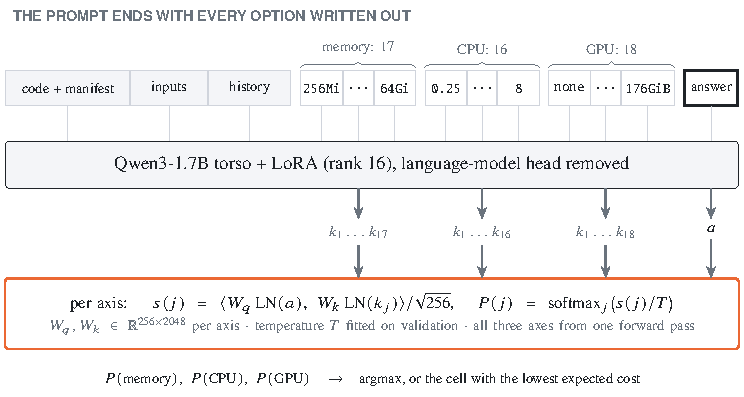
\includegraphics[width=\linewidth]{figures/diagrams/pointer.pdf}
\caption{The pointer decision model. Every prompt ends with the same options block and answer instruction, so
each option's last token sits at a fixed offset from the end, and one forward pass gives a distribution on all
three axes.}
\label{fig:pointer}
\end{figure}

The torso is Qwen3-1.7B~\citep{qwen3} without its language-model head, adapted with LoRA~\citep{hu2022lora}
(rank 16, $\alpha$ 32) on every projection of every layer. Prompts are cut from the left at 3,072 tokens, a length
no evaluated prompt reaches. The loss is the sum of the three axes' cross-entropies, leaving out memory and CPU for
GPU tasks. Training uses at most 5,000 rows per corpus and pod type, 27,936 rows in all, for one epoch with
micro-batches of 8, two accumulation steps, and AdamW at $2\times10^{-4}$ for the adapters and $10^{-3}$ for the
heads, on one NVIDIA L4. Two ablations train on one pod type only, on half the rows for two epochs, so that all
three variants take the same number of steps; each is calibrated on its own pod type's validation rows. The two
pod types are drawn independently, so the model trained on both sees about 40\% more distinct workloads than
either ablation.

\subsection{Turning a distribution into a request}
The trees, the decision models and the pools all give a distribution on each axis, and we read each one out in
two ways. The \emph{argmax} read-out takes the most likely cell on each axis. The \emph{decoded} read-out first
decides whether to give a GPU, choosing none when $P(\text{none})$ is at least a threshold $\theta$ tuned on
validation, and otherwise the most likely GPU cell. For memory it picks the cell with the lowest expected cost,
$\arg\min_m \sum_j C[m,j]\,P(j)$, where $C[m,j]$ is RightSizeMem's memory cost of requesting cell $m$ for a run
that needs cell $j$, retries included (a fixed matrix, not the per-run simulator). For CPU it picks the cell most
likely to fall within 25\% of the busiest window. An OOM costs a retry, so decoding leans toward asking for more
memory. For each model, validation decides which read-out the leaderboard reports (\cref{tab:readouts}).

\subsection{Reinforcement learning against the cost model}
Matching the label misses two things the cost model cares about. The axes interact: memory and CPU are free on
a GPU node, while a GPU is the most expensive mistake on a CPU node. And asking for too little costs more than
asking for too much. The RL approach starts from the decision model and maximizes the cost model's reward
(\cref{alg:grpo}). Because the policy is three categorical distributions, a group of 16 joint requests comes from
one forward pass and no text is generated. Advantages are normalized within each group as in
GRPO~\citep{shao2024deepseekmath}, and each batch takes one on-policy step, so the update is REINFORCE with a
group baseline and an exact KL penalty to the supervised model; there is no clipped ratio. It trains on 6,000
training prompts, about half of them unseen by the supervised model, for one epoch with a KL coefficient of 0.05
and the reward capped at 20.

The fitted temperatures of every RL model sit at or near the top of the search range (5.0), so its decoded
read-out is set by that bound. The RL policy moves probability away from the label cell on purpose, so
calibrating it against the label is the wrong target, and validation prefers its argmax read-out.

\begin{figure}[tbp]
\begin{lstlisting}
pi_ref = the supervised model's distributions, computed once before any update
for each batch of 8 prompts:
    one forward pass -> pi(.|x) on each axis
    sample K = 16 joint requests a^k = (m, c, g) from the three heads        # no text is generated
    r^k = - min( cost(x, a^k) / label_cost(x), 20 )                            # the benchmark's simulator
    A^k = (r^k - mean_k r) / (std_k r + 1e-3)                                  # group-normalized
    L   = - mean_k[ A^k * sum_{axis in S(x)} log pi(a^k_axis | x) ] + 0.05 * sum_{axis in S(x)} KL(pi || pi_ref)
    S(x) = {gpu} for a GPU task, else all three axes
\end{lstlisting}
\caption{RL without generation. The reward divides by a fixed cost per run, so the best request for each run is
the cheapest one whichever denominator is used. The KL term is exact over the categorical distributions.}
\label{alg:grpo}
\end{figure}

\subsection{Opinion pools}
The trees and the language models make different mistakes. The trees read numbers exactly and have nothing to go
on for code they have never seen; the language models read code well and treat numbers as tokens. A logarithmic
opinion pool~\citep{genest1986pools} combines their calibrated distributions on each axis:
\begin{equation}
p_{\text{pool}}(j) \propto p_{\text{trees}}(j)^{w}\,p_{\text{LM}}(j)^{1-w}.
\end{equation}
One weight $w$ is shared across the three axes and tuned on validation together with $\theta$, for the decoded
read-out; nothing is retrained. A model trained on one pod type is pooled with trees trained on the same pod type.

\subsection{A novelty gate}
In our first release, the pooled RL model read by argmax was the best approach on familiar code and one of the
worst on new code, while the RL model read out by decoding was the reverse. The gate sends each pod to one or the
other by its distance from the training data:
\begin{equation}
s(x) = \tfrac{1}{10}\textstyle\sum_{i=1}^{10}\lVert z(x) - z(x_{(i)})\rVert_2,\qquad
\text{request} = \begin{cases}\text{pool}\times\text{RL, argmax} & \text{if } s(x)\le\tau,\\ \text{RL, decoded} & \text{otherwise.}\end{cases}
\end{equation}
Here $z$ standardizes the trees' 209 features by their training mean and standard deviation, $x_{(i)}$ are the ten
nearest training pods, and $\tau$ is the 95th percentile of $s$ on validation. Validation has familiar families
only, so it cannot tune the gate: the threshold sends 5\% of familiar pods to the RL model by construction, and
validation regret falls steadily as fewer pods are routed. We chose the members, the signal and the threshold after
seeing the first release's unseen results, and fixed them before training k8s-2 at new seeds. k8s-2 has the same
seven held-out families, so it tests whether the choice holds up after relabelling and retraining, not whether it
generalizes to new families.

Our first release divided a feature that never varied in training by $10^{-9}$, so any pod with an unseen import
landed effectively infinitely far away. Such features now keep their raw units; the old scaling remains as a
comparison. We also compare two other signals: kNN on the 27 numeric features alone, and the Jensen--Shannon
divergence between the trees' and the RL model's predictions.

\subsection{A Flyte-to-Job adapter}
A team whose history is all Flyte tasks has no Job pods to train on. The adapter shifts a Flyte-trained model's
memory distribution with the accounting of \cref{sec:accounting}: each cell's representative need $n_j$ (its
geometric middle) becomes $(n_j/1.05 - R + 48[\text{boto3}] + B[\text{tmpfs}])\times1.05$, using the manifest's
volume medium, whether \code{job.py} imports boto3, and the input sizes. CPU and GPU come from the model's own
reading of the Job's prompt. Its memory distribution can come from the model's reading of the Job's prompt (the
variant a scheduler can deploy) or of the same run's Flyte task, which a scheduler holding only a raw Job does not
have. We report both.

\section{Experimental setup}
\label{sec:setup}

The whole benchmark runs as one Flyte factory on an EKS cluster: a graph of cached tasks,
each of which publishes a versioned artifact (\cref{fig:factory}). The trees and rules fit
on a CPU pod, each decision model and the RL model train on one NVIDIA L4, and the
zero-shot model runs as a shared vLLM service in the same cluster. Each of these is
itself a batch pod that someone had to size.

\begin{figure}[tbp]
\begin{lstlisting}
rt-bench-corpus[v2]   rt-cpubench-corpus[big-1]   rt-gpubench-corpus[big-2]        sources
      `---------------------+-----------------------------'
rt-k8sbench-corpus [release]              join_corpora: every run as a Job pod and a Flyte pod
      |-- rt-k8sbench-arm [release, arm]  fit_all_arm      CPU pod | hosted 27B | L4
      |-- rt-k8sbench-rl                  rl_all_policy    L4: decision model -> GRPO
      |-- rt-k8sbench-pool                pool_all_arms    trees x every decision model
      |-- rt-k8sbench-gate                gate_all_arms    kNN / numeric / disagreement gates, adapter
      |-- counterfactual                  staging_counterfactual, neutral names
rt-k8sbench-scorecard [release, arm]      score_all_arm    every split, pod type, staging, pair slice
rt-k8sbench-leaderboard [release]         all_leaderboard
\end{lstlisting}
\caption{The benchmark as a Flyte factory. Re-running it rebuilds only what changed.}
\label{fig:factory}
\end{figure}

We trained k8s-2 three times on the same data (\code{rsk-k8s-2}, \code{-s2} and
\code{-s3}). The seed controls data order, LoRA initialization and RL sampling. GPU kernels
are not bit-for-bit deterministic, so even the same seed would not reproduce a model
exactly. The zero-shot model is scored once, with seed 1. Unless we say otherwise, tables
show seed 1 with its bootstrap interval, and \cref{sec:res-seeds} reports the spread across
all three seeds. \Cref{app:runs} lists every cluster run.

\section{Results}
\label{sec:results}

\newcommand{\pairsN}{3,950}
\newcommand{\pairsMoved}{29.9}
\newcommand{\pairsUp}{638}
\newcommand{\pairsDown}{543}

\newcommand{\cfRuns}{1,189}
\newcommand{\cfRend}{4,756}
\newcommand{\cfMediumMovedTest}{48.6}
\newcommand{\cfMediumMovedOod}{74.2}
\newcommand{\cfFetchMovedTest}{20.4}
\newcommand{\cfFetchMovedOod}{18.8}


We report Job pods first, because they are the plain Kubernetes case, with no orchestrator to absorb mistakes.
Flyte pods follow, and so does the comparison between the two. Numbers are regret in percent against the cheapest
request, seed 1, with 95\% intervals clustered by task, unless noted.

\subsection{Leaderboard}
\label{sec:res-lead}

\Cref{tab:leaderboard,fig:tradeoff} give the main results. On new tasks from familiar families, the trees pooled
with the decision model are best at \rTestPoolDec\% \ciTestPoolDec. The trees pooled with the RL model and read by
argmax (\rTestPoolRLArg\%) cannot be separated from it (paired difference \vbTestPoolRLArg\ points
\vbTestPoolRLArgCI). The gate (\rTestGate\%) and RL read by argmax (\rTestRLArg\%) are about two points behind.
All four are ahead of the trees alone (\rTestTrees\%) and the decision model alone (\rTestDec\%), and far ahead of
the rules (\rTestSized\% for rules-sized, \rTestRules\% for rules) and the zero-shot model (\rTestZS\%). A static
request costs about twice the cheapest one.

On the seven held-out families every approach does worse, and the order changes. Rules-sized (\rUnseenSized\%) and
the gate (\rUnseenGate\%) have the lowest regret, and the gate equals the decoded RL model it routes those pods to.
The read-outs validation chose for the trained models do worse: RL read by argmax reaches \rUnseenRLArg\%, the
decision model \rUnseenDec\%, the pools \rUnseenPoolDec--\rUnseenPoolRLArg\%, and the trees \rUnseenTrees\%. The
zero-shot model is at \rUnseenZS\% on its smaller sample. Clustered by family, the intervals on this split are
wide: rules-sized spans \ciFamUnseenSized\ and RL read by argmax \ciFamUnseenRLArg, and of the approaches in
\cref{tab:leaderboard} only the static request is clearly worse than rules-sized.

\begin{table}[tbp]
\centering\small
\caption{Regret (\%) on Job pods for seed 1, with 95\% intervals clustered by task, and for the unseen split also
by family; regret on Flyte pods; dollar regret on Job pods; and the mean and range of Job regret over three
trainings. Each trained model is shown with the read-out validation chose (\cref{tab:readouts}). Bold marks the
approaches whose paired difference from the column's best includes zero. Each split has 5,095 Job pods for test
and 6,416 for unseen. $^\dagger$Zero-shot is scored on a sample of 130 test and 150 unseen Job pods
(\cref{tab:zs}) and is not compared for bold.}
\label{tab:leaderboard}
\resizebox{\linewidth}{!}{\begin{tabular}{@{}lrrrrrrrr@{}}
\toprule
& \multicolumn{2}{c}{Job pods: regret (\%)} & \multicolumn{2}{c}{Flyte pods} & \multicolumn{2}{c}{Job \$ regret} & \multicolumn{2}{c}{Job, 3 seeds: mean (range)} \\
\cmidrule(lr){2-3}\cmidrule(lr){4-5}\cmidrule(lr){6-7}\cmidrule(l){8-9}
approach & test & unseen & test & unseen & test & unseen & test & unseen \\
\midrule
static & 89.3\,{\scriptsize[84.7, 93.7]} & 115.1\,{\scriptsize[111.2, 119.2]} & 91.5 & 112.8 & 183.0 & 258.1 & 89.3 & 115.1 \\
rules & 42.4\,{\scriptsize[37.9, 46.7]} & 49.8\,{\scriptsize[47.0, 52.5]} & 41.3 & 48.0 & 56.9 & 120.3 & 42.4 & 49.8 \\
rules-sized & 37.7\,{\scriptsize[33.8, 41.6]} & \textbf{39.2}\,{\scriptsize[37.3, 41.2]} & 37.3 & 41.1 & 55.9 & 117.9 & 37.7 & 39.2 \\
zero-shot 27B & 48.8\,{\scriptsize[33.1, 67.2]} & 42.8\,{\scriptsize[29.6, 57.2]} & 35.7 & 52.0 & 86.0 & 30.0 & --- & --- \\
zero-shot 27B, JSON & 48.8\,{\scriptsize[31.9, 67.7]} & 44.4\,{\scriptsize[31.2, 59.2]} & 21.8 & 51.5 & 100.8 & 81.9 & --- & --- \\
trees & 11.5\,{\scriptsize[10.2, 12.8]} & 69.1\,{\scriptsize[66.3, 71.8]} & 14.6 & 69.0 & 30.6 & \textbf{85.6} & 11.5 & 69.1 \\
decision & 12.6\,{\scriptsize[11.3, 14.0]} & 47.8\,{\scriptsize[45.6, 50.4]} & 11.3 & 43.0 & 39.6 & 119.0 & 13.7\,{\scriptsize(12.6--15.0)} & 49.5\,{\scriptsize(44.2--56.6)} \\
decision, argmax & 30.3\,{\scriptsize[28.0, 32.5]} & 69.1\,{\scriptsize[66.2, 72.1]} & 28.7 & 63.8 & 39.8 & 107.2 & 30.8\,{\scriptsize(30.3--31.7)} & 72.6\,{\scriptsize(68.1--80.6)} \\
RL & 14.6\,{\scriptsize[13.2, 16.1]} & 39.3\,{\scriptsize[37.3, 41.4]} & 14.3 & \textbf{40.2} & 50.6 & 127.9 & 16.2\,{\scriptsize(14.6--17.4)} & 37.7\,{\scriptsize(35.5--39.3)} \\
RL, argmax & 8.5\,{\scriptsize[7.1, 9.9]} & 46.5\,{\scriptsize[44.2, 48.8]} & 8.6 & 46.2 & 35.3 & 106.4 & 8.4\,{\scriptsize(8.2--8.6)} & 45.0\,{\scriptsize(41.3--47.2)} \\
pool $\times$ decision & \textbf{6.6}\,{\scriptsize[5.6, 7.6]} & 56.8\,{\scriptsize[54.5, 59.2]} & \textbf{5.5} & 51.4 & 27.6 & 95.0 & 6.8\,{\scriptsize(6.6--6.9)} & 55.7\,{\scriptsize(52.1--58.3)} \\
pool $\times$ RL & 10.5\,{\scriptsize[9.4, 11.8]} & 49.6\,{\scriptsize[47.5, 51.8]} & 11.1 & 50.3 & 34.7 & 100.8 & 10.7\,{\scriptsize(10.5--11.0)} & 53.9\,{\scriptsize(49.6--61.3)} \\
pool $\times$ RL, argmax & 7.2\,{\scriptsize[6.0, 8.4]} & 79.4\,{\scriptsize[75.7, 83.2]} & 7.1 & 78.1 & \textbf{15.7} & 111.6 & 8.6\,{\scriptsize(6.8--11.8)} & 89.6\,{\scriptsize(78.6--110.9)} \\
gate (kNN, $q$ 0.95) & 8.1\,{\scriptsize[6.9, 9.4]} & 39.3\,{\scriptsize[37.3, 41.4]} & 7.6 & \textbf{40.2} & 19.5 & 127.9 & 9.6\,{\scriptsize(8.1--12.7)} & 37.7\,{\scriptsize(35.5--39.3)} \\
\bottomrule
\end{tabular}
}
\end{table}

\begin{figure}[tbp]
\centering
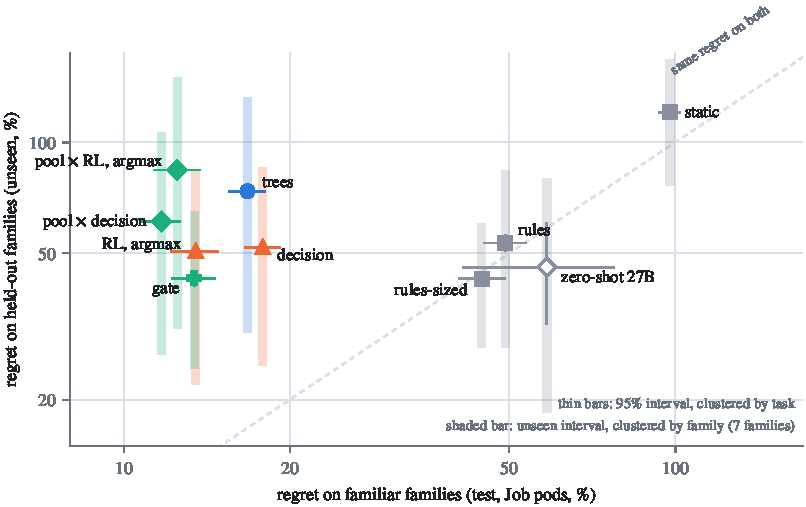
\includegraphics[width=\linewidth]{figures/fig_tradeoff.pdf}
\caption{Regret on familiar families against regret on held-out families, Job pods, seed 1 (log scales). Gray:
static request, rules and zero-shot (hollow: scored on a sample). Blue: trees. Orange: language models. Green:
pools and the gate. No approach is in the lower left: the approaches that lead on familiar code fall behind a
sized rule on new code.}
\label{fig:tradeoff}
\end{figure}

The gate is the only trained approach near the top on both splits, at a cost of
\diffTestGatePoolRLArg\ points on familiar code \diffTestGatePoolRLArgCI\ against its familiar-code member and a
saving of \diffUnseenGatePoolRLArg\ points on new code \diffUnseenGatePoolRLArgCI. It does not beat rules-sized on
new code (\diffUnseenSizedGate\ points \diffUnseenSizedGateCI), and its members were chosen with the same held-out
families in view (\cref{sec:res-gate}).

\subsection{Seen code, new programs and new families}
\label{sec:res-code}

Most familiar-family test tasks are programs the models have seen. \codeSeenShare\% of test Job pods run code
identical to a training task's, and differ only in input sizes and history. \Cref{tab:code} splits the test split
in two. On the \codeNovelN{} pods with new programs, regret rises for every trained approach. The decision model
goes from \seenDec\% to \novelDec\%. The trees pooled with the RL model and read by argmax barely move
(\seenPoolRLArg\% to \novelPoolRLArg\%), and the gate goes from \seenGate\% to \novelGate\%. The held-out families
are the larger step: new programs from familiar families stay within 13--35\% of the cheapest request, while every approach is at about 43\% or worse on the new
families. Rules-sized reads only sizes and the pod spec, so it is the same on both halves.

\begin{table}[tbp]
\centering\small
\caption{Job regret (\%) on test pods whose task code appears in training (seen) and on those whose code does
not (new), with the unseen families for comparison, for seed 1.}
\label{tab:code}
\begin{tabular}{@{}lrrr@{}}
\toprule
& \multicolumn{2}{c}{test: code in training?} & \\
\cmidrule(lr){2-3}
approach & seen (4,135) & new (960) & unseen families \\
\midrule
static & 86.1 & 148.0 & 120.7 \\
rules & 52.0 & 36.7 & 53.3 \\
rules-sized & 44.5 & 44.4 & 42.7 \\
trees & 15.7 & 21.4 & 73.8 \\
decision & 14.0 & 34.3 & 51.9 \\
RL, argmax & 11.6 & 21.8 & 50.6 \\
pool $\times$ decision & 10.3 & 17.9 & 61.0 \\
pool $\times$ RL, argmax & 12.4 & 13.2 & 84.1 \\
gate & 12.6 & 16.8 & 42.8 \\
\bottomrule
\end{tabular}

\end{table}

Part of the gap between test and unseen comes from the corpus mix: GPU runs are 36\% of unseen pods and 22\% of
test pods. \Cref{tab:corpus} in \cref{app:extra} breaks results down by corpus. The trees' weakness on new code is
concentrated in CPU and GPU families (\cUnseenCpuTrees\% and \cUnseenGpuTrees\%), and rules-sized is strongest on the
held-out CPU families (\cUnseenCpuSized\%).

\subsection{Does a model need to see Jobs?}
\label{sec:res-training}

\Cref{tab:training} trains the trees, the decision model and the pool three ways: on both pod types, on Jobs alone,
and on Flyte tasks alone. Flyte data does not make the models better on Jobs. A decision model trained only on Jobs
scores \rTestDecJob\% on Job test pods, against \rTestDec\% for one trained on both, a difference of
\diffTestDecDecJob\ points \diffTestDecDecJobCI; on seed 3 the Job-only model is better. The trees and the pool
behave the same way. The reverse transfer does not work. A model trained only on Flyte tasks scores \rTestDecFlyte\%
on Job pods, and the pool built on it reaches \rTestPoolDecFlyte\% where the pool trained on both reaches
\rTestPoolDec\%. A model trained only on Jobs also does worse on Flyte pods (\rFTestDecJob\% against \rFTestDec\%),
by less, because a Flyte task is closer to a Job with a small fixed runtime added than the other way around. On the
unseen families, the model trained on both pod types is ahead by \diffUnseenDecDecJob\ points
\diffUnseenDecDecJobCI, which may reflect the larger number of distinct workloads it saw.

\begin{table}[tbp]
\centering\small
\caption{What the training data includes. Regret (\%) on Job and Flyte pods, and the share of Job pods whose first
attempt succeeds, for seed 1.}
\label{tab:training}
\begin{tabular}{@{}llrrrrr@{}}
\toprule
&& \multicolumn{2}{c}{Job pods: regret (\%)} & \multicolumn{2}{c}{Flyte pods: regret (\%)} & Job \\
\cmidrule(lr){3-4}\cmidrule(lr){5-6}
approach & trained on & test & unseen & test & unseen & first OK \\
\midrule
trees & both & 11.5\,{\scriptsize[10.2, 12.8]} & 69.1 & 14.6\,{\scriptsize[13.3, 16.1]} & 69.0 & 97.6 \\
 & Jobs only & 11.8\,{\scriptsize[10.5, 13.1]} & 68.6 & 26.2\,{\scriptsize[24.4, 28.0]} & 78.9 & 97.7 \\
 & Flyte only & 18.3\,{\scriptsize[16.8, 19.9]} & 73.5 & 15.9\,{\scriptsize[14.5, 17.3]} & 93.5 & 94.1 \\
\midrule
decision & both & 12.6\,{\scriptsize[11.3, 14.0]} & 47.8 & 11.3\,{\scriptsize[10.0, 12.6]} & 43.0 & 97.2 \\
 & Jobs only & 13.2\,{\scriptsize[11.8, 14.7]} & 56.1 & 20.5\,{\scriptsize[18.8, 22.3]} & 53.6 & 97.0 \\
 & Flyte only & 37.3\,{\scriptsize[35.1, 39.6]} & 59.0 & 12.0\,{\scriptsize[10.6, 13.5]} & 48.5 & 87.2 \\
\midrule
decision, argmax & both & 30.3\,{\scriptsize[28.0, 32.5]} & 69.1 & 28.7\,{\scriptsize[26.5, 31.0]} & 63.8 & 87.3 \\
 & Jobs only & 28.8\,{\scriptsize[26.7, 31.1]} & 74.4 & 41.4\,{\scriptsize[38.8, 44.0]} & 79.3 & 87.0 \\
 & Flyte only & 56.2\,{\scriptsize[53.3, 59.3]} & 84.4 & 27.5\,{\scriptsize[25.4, 29.6]} & 66.6 & 76.9 \\
\midrule
pool $\times$ decision & both & 6.6\,{\scriptsize[5.6, 7.6]} & 56.8 & 5.5\,{\scriptsize[4.6, 6.6]} & 51.4 & 98.3 \\
 & Jobs only & 7.7\,{\scriptsize[6.6, 8.8]} & 57.9 & 17.1\,{\scriptsize[15.6, 18.6]} & 58.7 & 98.0 \\
 & Flyte only & 24.8\,{\scriptsize[22.9, 26.7]} & 51.6 & 5.4\,{\scriptsize[4.4, 6.5]} & 49.6 & 91.3 \\
\bottomrule
\end{tabular}

\end{table}

A model trained on both pod types treats them almost the same. The paired difference between a run's Job pod and
its Flyte pod is under two points on familiar code for every language model and pool (\cref{tab:gap}), and for the
RL model it is indistinguishable from zero; the trees do 3.0 points better on Jobs. On new code, the decision model and
its pool do about five points worse on Jobs than on Flyte tasks, while RL and the gate do about a point better.

\paragraph{The adapter.}
The adapter of \cref{sec:methods} shifts a Flyte-trained model's memory distribution through the staging
accounting. The variant that reads the run's Flyte task cuts the Flyte-only model's Job regret from
\rTestDecFlyte\% to \rTestDecAdapt\% on seed 1, from 40.1\% to 28.1\% on seed 2, and from 44.2\% to 34.9\% on seed 3.
The variant a scheduler can deploy, which reads only the Job's prompt, does not help (44.9\%, 40.2\% and 43.4\%),
though pooling it with Flyte-trained trees does (29.6\%, 26.1\% and 26.9\%). Either way the adapter stays well short
of a model that has seen Jobs (17--20\%): platform data matters even when the accounting is known.

\subsection{Does a model read the manifest?}
\label{sec:res-manifest}

A model could do well on Jobs by learning only that a Job's numbers run lower than a Flyte task's, because a Job
does not carry the runtime. We test this two ways.

\paragraph{Run and Job pairs.}
Of the \pairsN{} test pairs of a run's Flyte pod and its Job pod on CPU nodes, the memory label differs in
\pairsMoved\%. In \pairsUp{} pairs the Job needs more, because it stages its inputs on tmpfs, and in \pairsDown{} it
needs less, because it has no runtime. A model that ignores the pod type keeps the same request for both pods,
which scores 100\% on the pairs whose label stays the same and 0\% on those whose label moves. Models trained on
both pod types move the right way on 56--67\% of the pairs that move, and on 75--83\% of upward moves
(\cref{tab:pairs}). The rules move the right way on 25\%.

\paragraph{A controlled counterfactual.}
The pairs above mix the effect of the manifest with the effect of the runtime. To isolate the manifest, we took
\cfRuns{} first runs from the test and unseen splits and rendered each one as a Job under all four stagings,
holding the task, code and inputs fixed (\cfRend{} pods). Only the manifest and the way the job fetches its inputs
change, and with no history, the manifest is the only evidence of the staging. Switching the volume from disk to
tmpfs moves the label in \cfMediumMovedTest\% of test pairs and \cfMediumMovedOod\% of unseen pairs, and switching
the fetcher from an init container to boto3 moves it in about a fifth.

\begin{figure}[tbp]
\centering
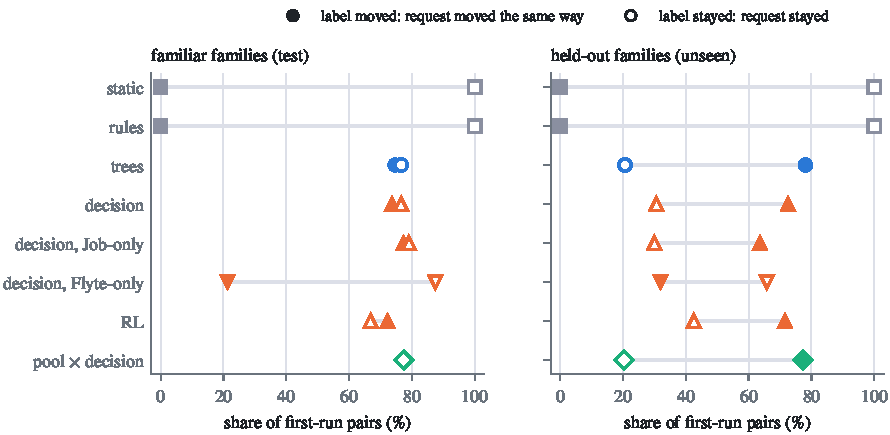
\includegraphics[width=\linewidth]{figures/fig_counterfactual.pdf}
\caption{The staging counterfactual, seed 1: the same first runs rendered as Jobs with the inputs on node disk and
on a memory-backed volume. Filled: among pairs whose label moved, the share where the request moved the same way.
Hollow: among pairs whose label stayed, the share where the request stayed too. Static requests and rules never
move on a first run.}
\label{fig:counterfactual}
\end{figure}

The models trained on Jobs read the manifest (\cref{fig:counterfactual,tab:cf}). When the label moves, the
decision model, the trees, RL and the pools move their request the right way on 72--78\% of familiar-code pairs and
64--78\% of unseen pairs. The Flyte-only model, which has never seen a manifest, does so on 21\%. Static requests and
rules never move, because on a first run they have only fixed defaults. On new code the models overreact: when the
label does not move, which mostly means the staged inputs were small, they still change their request on 57--80\% of
unseen pairs. They pick up the fetcher less reliably (31--47\% on test), which fits boto3's 48\,MiB only sometimes
crossing a cell.

\paragraph{The task's name.}
Generated tasks are named after their family (for example \code{pandas-join}), and the name appears in the code and
the manifest. We re-scored the counterfactual's first runs with each name replaced by a hash, without retraining
(\cref{tab:names}). On familiar code, regret changes by less than a point for every trained approach except the
Flyte-only model (+1.8); on new code it rises by 0.5--3.6 points. Each family also has a fixed function name and
input schema, which this test leaves in place, so it bounds the name's effect without removing the family's
identity from the code.

\subsection{The gate}
\label{sec:res-gate}

\Cref{tab:gate} compares the gate's signal with the alternatives. Correcting the first release's kNN scaling changed
nothing: the corrected distance still separates unseen families from validation with an AUROC of 0.999, sends every
unseen pod to RL, and gives exactly the same requests. The held-out families are far from the training data in code
tokens, though only one of them imports a library no training family uses (\cref{sec:dataset}). With code tokens
removed the AUROC falls to 0.67 and unseen regret rises to 66.4\%. The detector's job is easy on this
benchmark, and the benchmark cannot test it on new code built from familiar tokens.

\begin{table}[tbp]
\centering\small
\caption{Gate signals for seed 1. AUROC measures how well each signal ranks unseen pods above validation pods. The
middle columns give the share of pods routed to the RL model, and the last two the gate's regret on Job pods. All
gates use the 0.95 quantile except the disagreement gate, shown at 0.5.}
\label{tab:gate}
\begin{tabular}{@{}lrrrrr@{}}
\toprule
&& \multicolumn{2}{c}{sent to RL (\%)} & \multicolumn{2}{c}{Job regret (\%)} \\
\cmidrule(lr){3-4}\cmidrule(l){5-6}
signal & AUROC & test & unseen & test & unseen \\
\midrule
kNN, all features & 0.999 & 5.3 & 100.0 & 8.1\,{\scriptsize[7.0, 9.4]} & 39.3\,{\scriptsize[37.3, 41.3]} \\
kNN, k8s-1 scaling & 1.000 & 5.3 & 100.0 & 8.1\,{\scriptsize[7.0, 9.4]} & 39.3\,{\scriptsize[37.1, 41.4]} \\
kNN, numeric only & 0.673 & 4.5 & 30.5 & 7.9\,{\scriptsize[6.7, 9.2]} & 61.9\,{\scriptsize[59.0, 64.7]} \\
disagreement (JS), $q$ 0.5 & 0.729 & 51.3 & 80.5 & 11.5\,{\scriptsize[10.2, 13.0]} & 42.9\,{\scriptsize[40.8, 45.0]} \\
\bottomrule
\end{tabular}

\end{table}

Over three trainings, the gate averages \mTestGate\% on familiar code (\loTestGate--\hiTestGate\%) and
\mUnseenGate\% on new code (\loUnseenGate--\hiUnseenGate\%). Seed 3's familiar-code number is higher because its
familiar-code member, the pooled RL model read by argmax, was worse on that seed (17.5\%). On new code the gate always
equals the decoded RL model, whose temperature sits at its search bound (\cref{sec:methods}); validation would have
chosen that model's argmax read-out, which is about eight points worse on new code (\diffUnseenRLArgRL\ points
\diffUnseenRLArgRLCI).

\subsection{First runs and runs with history}
\label{sec:res-cold}

First runs are where the approaches differ most (\cref{tab:cold}). With history, most trained approaches do well on
familiar code (6--13\%), and rules-sized reaches 16.8\%. On first runs the rules lose most of their accuracy
(72--82\%), while the pooled decision model holds at 16.4\%. On new code, history does most of the work, and
rules-sized with history (16.9\%) is the best of any approach, because scaling the nearest earlier run by input size is a strong prior when a task's runs
differ only in size. Without history, no approach does well on new code; the best are the zero-shot model, on its
sample, and the gate.

\begin{table}[tbp]
\centering\small
\caption{Job regret (\%) on first runs and on runs with history, for seed 1.}
\label{tab:cold}
\begin{tabular}{@{}lrrrr@{}}
\toprule
& \multicolumn{2}{c}{test} & \multicolumn{2}{c}{unseen} \\
\cmidrule(lr){2-3}\cmidrule(l){4-5}
approach & first run & with history & first run & with history \\
\midrule
static & 107.7 & 90.4 & 137.4 & 106.2 \\
rules & 74.7 & 30.0 & 77.0 & 32.8 \\
rules-sized & 81.5 & 16.8 & 72.4 & \textbf{16.9} \\
zero-shot 27B & 98.0 & 24.6 & 59.6 & 36.1 \\
zero-shot 27B, JSON & 88.5 & 31.8 & 81.2 & 22.9 \\
trees & 22.0 & 12.9 & 115.5 & 37.6 \\
decision & 27.5 & 10.7 & 81.7 & 26.1 \\
RL, argmax & 23.2 & \textbf{6.2} & 80.5 & 24.6 \\
pool $\times$ decision & \textbf{16.4} & 8.2 & 103.9 & 23.8 \\
pool $\times$ RL, argmax & 19.3 & 7.4 & 145.9 & 30.6 \\
gate & 20.3 & 8.3 & \textbf{65.2} & 23.3 \\
\bottomrule
\end{tabular}

\end{table}

\subsection{Dollars and the price of a retry}
\label{sec:res-sens}

Mean regret counts every pod equally, while dollar regret is dominated by large jobs. On familiar code the two
mostly agree: the pooled RL model read by argmax costs \dTestPoolRLArg\% more than the cheapest requests in total,
and the gate \dTestGate\%. On new code, dollars rank the trees first (\dUnseenTrees\%), because they size the largest
jobs better even though their mean regret is among the worst. The trees cost \$\usdUnseenTrees{} per 1,000 unseen Job
runs, against \$\usdUnseenSized{} for rules-sized, \$\usdUnseenGate{} for the gate, and \$\usdCheapUnseen{} for the
cheapest requests.

A raw Job with \code{backoffLimit: 0} does not retry: it fails, and someone resubmits it. That makes an OOM much more
expensive than our default penalty. \Cref{fig:penalty,tab:sens} re-score every approach with penalties of 0, 5 and
20 times the label request's cost per retry. Every approach was tuned at the default penalty of 1, so this measures
how fixed requests hold up when failures get dearer, not how well each approach could adapt. On familiar code the
pooled decision model has the lowest regret at every penalty from 1 to 20 (\pTwentyTestPoolDec\% at 20), though at 20
the pooled RL model is within \sdTwentyTestPoolDecPoolRLArg{} points \sdTwentyTestPoolDecPoolRLArgCI. On new code,
rules-sized has the lowest regret at penalties of 5 and 20 (\pFiveUnseenSized\% and \pTwentyUnseenSized\%), ahead of RL
and the gate (\pFiveUnseenRL\% and \pTwentyUnseenGate\%). Clustered by task, that lead is clear
(\sdTwentyUnseenSizedGate\ points \sdTwentyUnseenSizedGateCI\ at 20); clustered by the seven families, it is not
(\sdFamTwentyUnseenSizedGateCI). For teams that run raw Jobs without retries, the evidence favours a rule that scales
by input size and reads the manifest on code nobody has seen before, and does not rule out the trained models.

\begin{figure}[tbp]
\centering
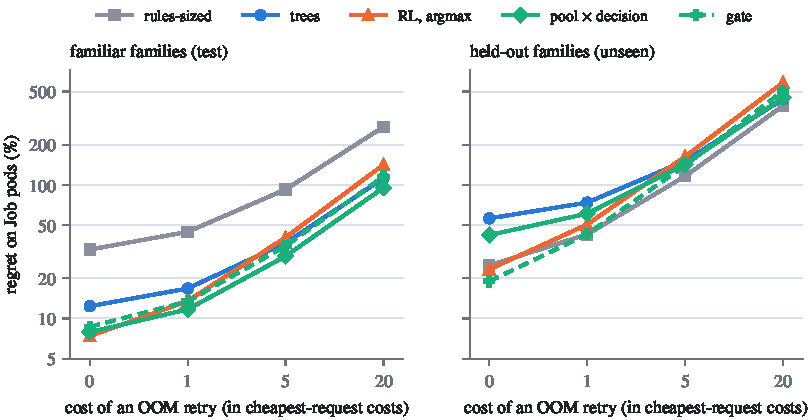
\includegraphics[width=\linewidth]{figures/fig_penalty.pdf}
\caption{Job regret as an OOM retry gets more expensive, seed 1 (log scale). Every approach was tuned at a penalty
of 1. On familiar code the trained approaches stay far ahead of rules-sized; on held-out families the lines cross,
and rules-sized has the lowest regret once a retry costs 5 or more.}
\label{fig:penalty}
\end{figure}

\begin{table}[tbp]
\centering\small
\caption{Job regret (\%) when each OOM retry costs 0, 1 (the default), 5 or 20 times the label request's cost.
Higher penalties stand for a Job that fails outright and has to be resubmitted.}
\label{tab:sens}
\resizebox{\linewidth}{!}{\begin{tabular}{@{}lrrrrrrrr@{}}
\toprule
& \multicolumn{2}{c}{0} & \multicolumn{2}{c}{1 (default)} & \multicolumn{2}{c}{5} & \multicolumn{2}{c}{20} \\
\cmidrule(lr){2-3}\cmidrule(lr){4-5}\cmidrule(lr){6-7}\cmidrule(l){8-9}
approach & test & unseen & test & unseen & test & unseen & test & unseen \\
\midrule
static & 47.8 & 44.3 & 89.3 & 115.1 & 255.2 & 398.2 & 877.6 & 1459.9 \\
rules & 28.8 & 24.7 & 42.4 & 49.8 & 96.9 & 149.9 & 301.2 & 525.6 \\
rules-sized & 25.9 & 20.9 & 37.7 & \textbf{39.2} & 84.9 & \textbf{112.5} & 261.8 & \textbf{387.2} \\
zero-shot 27B & 31.1 & 18.8 & 48.8 & 42.8 & 119.5 & 138.8 & 384.9 & 498.8 \\
zero-shot 27B, JSON & 26.5 & 24.4 & 48.8 & 44.4 & 138.0 & 124.4 & 472.6 & 424.4 \\
trees & 6.5 & 50.8 & 11.5 & 69.1 & 31.4 & 142.5 & 105.8 & 417.7 \\
decision & 7.3 & 20.2 & 12.6 & 47.8 & 33.8 & 158.6 & 113.3 & 573.8 \\
decision, argmax & 17.8 & 35.2 & 30.3 & 69.1 & 80.6 & 204.8 & 269.0 & 713.5 \\
RL & 8.1 & \textbf{15.2} & 14.6 & 39.3 & 40.4 & 135.7 & 137.3 & 497.1 \\
RL, argmax & \textbf{1.9} & 19.1 & 8.5 & 46.5 & 35.0 & 156.1 & 134.6 & 567.1 \\
pool $\times$ decision & 2.3 & 37.0 & \textbf{6.6} & 56.8 & \textbf{24.0} & 135.9 & \textbf{89.4} & 432.6 \\
pool $\times$ RL & 5.6 & 31.0 & 10.5 & 49.6 & 30.4 & 124.0 & 104.9 & 403.2 \\
pool $\times$ RL, argmax & 2.3 & 54.3 & 7.2 & 79.4 & 26.9 & 179.6 & 100.8 & 555.6 \\
gate (kNN, $q$ 0.95) & 2.9 & \textbf{15.2} & 8.1 & 39.3 & 29.1 & 135.7 & 107.7 & 497.1 \\
\bottomrule
\end{tabular}
}
\end{table}

\subsection{Three trainings}
\label{sec:res-seeds}

The static request, both rules and the trees give identical results on every seed. The trained models vary, more on
new code than on familiar code (\cref{tab:seeds}). On familiar code the top is stable: the pooled decision model ranges
from \loTestPoolDec\% to \hiTestPoolDec\% and RL read by argmax from \loTestRLArg\% to \hiTestRLArg\%. The pooled RL
model read by argmax ranges from \loTestPoolRLArg\% to \hiTestPoolRLArg\%. On new code, the decision model ranges from
\loUnseenDec\% to \hiUnseenDec\% and the pooled RL model read by argmax from \loUnseenPoolRLArg\% to
\hiUnseenPoolRLArg\%, while the gate varies least (\loUnseenGate--\hiUnseenGate\%). Rankings on new code within about
ten points of each other are not stable across trainings.

\begin{table}[tbp]
\centering\small
\caption{Job regret (\%) for each of the three trainings. The static request, the rules and the trees give identical
results on every seed.}
\label{tab:seeds}
\begin{tabular}{@{}lrrrrrr@{}}
\toprule
& \multicolumn{3}{c}{Job test, by seed} & \multicolumn{3}{c}{Job unseen, by seed} \\
\cmidrule(lr){2-4}\cmidrule(l){5-7}
approach & 1 & 2 & 3 & 1 & 2 & 3 \\
\midrule
static & 89.3 & 89.3 & 89.3 & 115.1 & 115.1 & 115.1 \\
rules & 42.4 & 42.4 & 42.4 & 49.8 & 49.8 & 49.8 \\
rules-sized & 37.7 & 37.7 & 37.7 & 39.2 & 39.2 & 39.2 \\
trees & 11.5 & 11.5 & 11.5 & 69.1 & 69.1 & 69.1 \\
decision & 12.6 & 13.4 & 15.0 & 47.8 & 44.2 & 56.6 \\
decision, argmax & 30.3 & 30.3 & 31.7 & 69.1 & 68.1 & 80.6 \\
RL & 14.6 & 16.7 & 17.4 & 39.3 & 38.2 & 35.5 \\
RL, argmax & 8.5 & 8.6 & 8.2 & 46.5 & 47.2 & 41.3 \\
pool $\times$ decision & 6.6 & 6.8 & 6.9 & 56.8 & 52.1 & 58.3 \\
pool $\times$ RL & 10.5 & 10.5 & 11.0 & 49.6 & 50.9 & 61.3 \\
pool $\times$ RL, argmax & 7.2 & 6.8 & 11.8 & 79.4 & 78.6 & 110.9 \\
gate (kNN, $q$ 0.95) & 8.1 & 8.1 & 12.7 & 39.3 & 38.2 & 35.5 \\
decision, Job-only & 13.2 & 13.8 & 12.2 & 56.1 & 53.3 & 68.5 \\
decision, Flyte-only & 37.3 & 33.8 & 37.5 & 59.0 & 67.1 & 76.1 \\
trees, Job-only & 11.8 & 11.8 & 11.8 & 68.6 & 68.6 & 68.6 \\
trees, Flyte-only & 18.3 & 18.3 & 18.3 & 73.5 & 73.5 & 73.5 \\
\bottomrule
\end{tabular}

\end{table}

\subsection{Zero-shot}
\label{sec:res-zs}

With room to finish its reasoning, the 27B model answers almost every prompt. \Cref{tab:zs} scores every approach on
the zero-shot model's own sample, so the comparison is like for like. On familiar code the zero-shot model
(\zsTestZS\%) is worse than the rules (\zsTestRules\% and \zsTestSized\%; paired difference with rules-sized
\diffTestZSSized\ points \diffTestZSSizedCI) and far behind the trained models (\zsTestRLArg\% for RL read by argmax). On
new code it is level with the best approaches on that sample (\zsUnseenZS\% against \zsUnseenSized\% for rules-sized and
\zsUnseenGate\% for the gate), with intervals of about $\pm$15 points. Constraining it to the JSON schema makes little
difference on Jobs and helps on Flyte tasks (\rFTestZSJ\% on familiar code).

\section{Discussion}
\label{sec:discussion}

\paragraph{Benchmarking Kubernetes pods from one set of measurements.}
Because the user code is the same whichever way a pod is submitted, one measurement of
the workload can label both a raw Job and a Flyte task, as long as the accounting for the
pod's edges is right. Getting it right took real pods. Sibling processes in one pod
confirmed the arithmetic, but only per-container cgroups showed where tmpfs pages are
charged, that the first release's init containers could not hold their inputs, and that
the Flyte runtime was less than half the size we had assumed. Anyone deriving Kubernetes
labels this way should check them against the cgroup, not against another RSS
measurement.

\paragraph{What a model learns from Jobs.}
A model trained on Jobs reads the manifest. It changes its memory request when the
volume medium changes, and it does so on first runs where nothing else gives the staging
away. Flyte tasks add nothing to that model's accuracy on Jobs, and a Flyte-only model
does not transfer well even after an explicit adapter. For a team that submits pods both
ways, the practical advice is to train on the pods it actually runs. Flyte history is still
useful for sizing Flyte tasks, and the corrected adapter recovers part of the gap when Job
history is missing.

\paragraph{Familiar and unfamiliar code.}
The gap between the two splits is the main open problem. On familiar code the best
approaches are within 7--8\% of the oracle. On new kinds of code, the best trained model is
39\% above it, and a careful rule matches it. Pooling the trees with a language model helps
on familiar code and hurts on new code, because the pool's weight is tuned on familiar
families. The gate recovers the better of the two on each split, but on this benchmark its
detector has an easy job, since new families usually bring new libraries. A benchmark
that separates unfamiliar code from unfamiliar libraries would test it properly.

\paragraph{Cost, not accuracy.}
Accuracy on the label and cost often disagree. Cost-aware decoding over-asks on purpose,
the Flyte-to-Job adapter was judged a failure until its runtime constant was corrected, and
the ranking on new code flips when retries become expensive. A benchmark for this
decision has to score money, and it has to say what a failure costs.

\section{Limitations}
\label{sec:limitations}

The workloads are synthetic. They use real libraries and real code paths, but the tasks
are generated, the data is random, and runs take seconds to minutes. Production tasks are
longer and messier. The seven unseen families were chosen by hand, and six of them
introduce a library that no training family uses, so the benchmark does not test new code
built only from familiar libraries. The people who wrote the generators also wrote the tree
features and the rules, and the task names give away the family, although removing them
changes regret by less than four points.

The labels carry three known biases. The \code{ru\_maxrss} floor and memory-mapped inputs
make about a third of labels one cell larger than strictly needed, so the oracle is
slightly generous. Process pools are labelled by their largest process rather than their
total, which is why two of 100 real pods failed at their label. And RightSizeMem has no
per-second CPU series, so its throttling is modelled from mean cores. The Job labels are
derived rather than measured for every run. We validated them on 100 runs in real pods
and 176 in a single pod, but we did not re-measure GPU runs as Jobs, and the four stagings
leave out sidecars, CSI drivers and other init work.

The cost model uses list prices, with no spot discounts or bin-packing, and prices a retry
at one oracle cost by default; \cref{sec:res-sens} shows how much that choice matters. We
trained three times, which shows that rankings on new code within about ten points are not
stable, but three seeds are not enough to put tight intervals on that variation. The
zero-shot model was scored on a sample of about 300 runs per split, and only once.

\section{Conclusion}
\label{sec:conclusion}

RightSize Bench scores the request a scheduler makes before a Kubernetes pod runs, in
dollars, across 33 families of task code submitted both as raw Jobs and through Flyte.
Checking its labels in real pods fixed two errors and measured the cost of Flyte's runtime
at about 70\,MiB. A small model trained on Jobs reads the manifest and, pooled with
gradient-boosted trees, comes within 7\% of the oracle on familiar code. On unfamiliar
code, the best trained model and a careful rule are both about 39\% above the oracle, and
the rule is safer when failures are expensive. Closing that gap, and testing a novelty
detector on code that looks familiar but is not, is the work that remains.


\bibliographystyle{plainnat}
\bibliography{refs}

\appendix
\section{Task families}
\label{app:families}

\Cref{tab:families} lists every family with its resource driver and one sample input,
rendered as an approach sees it (seed 7). ``Unseen'' families are held out of training
and validation. ``Sharded'' families spread over every visible GPU. Lines is the
length of the sample's function body.

\begin{table}[h]
\centering\small
\caption{The 33 task families.}
\label{tab:families}
\resizebox{\linewidth}{!}{\begin{tabular}{@{}llllr@{}}
\toprule
corpus & family & driver & sample input & lines \\
\midrule
RightSizeMem & \code{csv\_chunked} & code & {\scriptsize\ttfamily readings: csv, header: device,x0,x1,x2,x3,x4,x5,x6,x7,tag0} & 13 \\
 & \code{jsonl\_records} & both & {\scriptsize\ttfamily logs: jsonl, first record keys: ['user', 'score0', 'scor\ldots} & 17 \\
 & \code{numpy\_linalg} & both & {\scriptsize\ttfamily matrix: npy, shape=(326345, 128), dtype=float64} & 15 \\
 & \code{pandas\_groupby} & both & {\scriptsize\ttfamily events: parquet, 1,790,583 rows, schema=[customer\_id: i\ldots} & 14 \\
 & \code{pandas\_join} & both & {\scriptsize\ttfamily orders: parquet, 632,344 rows, schema=[order\_id: int64,\ldots} & 19 \\
 & \code{polars\_pipeline} & code & {\scriptsize\ttfamily events: parquet, 2,236,012 rows, schema=[user\_id: int64\ldots} & 15 \\
 & \code{python\_grouping} & both & {\scriptsize\ttfamily rows: csv, header: key,value,note0,note1,note2} & 18 \\
 & \code{sklearn\_fit} & both & {\scriptsize\ttfamily train: parquet, 326,345 rows, schema=[x0: double, x1: do\ldots} & 19 \\
 & \code{tfidf\_text} & both & {\scriptsize\ttfamily docs: parquet, 52,765 rows, schema=[doc\_id: int64, text\ldots} & 16 \\
 & \code{torch\_train} & both & {\scriptsize\ttfamily train: parquet, 1,710,807 rows, schema=[x0: double, x1:\ldots} & 39 \\
 & \code{duckdb\_sql (unseen)} & code & {\scriptsize\ttfamily events: parquet, 2,403,570 rows, schema=[account\_id: in\ldots} & 15 \\
 & \code{image\_batch (unseen)} & both & {\scriptsize\ttfamily images: npy, shape=(52998, 128, 128, 3), dtype=uint8} & 15 \\
\midrule
RightSizeCPU & \code{io\_bound} & io & {\scriptsize\ttfamily events: jsonl, first record keys: ['user', 'event', 'pay\ldots} & 27 \\
 & \code{mixed\_phases} & phases & {\scriptsize\ttfamily matrix: npy, shape=(101438, 256), dtype=float64} & 28 \\
 & \code{numpy\_blas} & threads & {\scriptsize\ttfamily features: npy, shape=(135042, 512), dtype=float32} & 25 \\
 & \code{pandas\_serial} & serial & {\scriptsize\ttfamily orders: parquet, 893,225 rows, schema=[customer\_id: int\ldots} & 20 \\
 & \code{polars\_groupby} & threads & {\scriptsize\ttfamily events: parquet, 5,464,904 rows, schema=[key: int64, reg\ldots} & 22 \\
 & \code{process\_pool} & processes & {\scriptsize\ttfamily docs: csv, header: id,text} & 31 \\
 & \code{python\_threadpool} & gil & {\scriptsize\ttfamily blob: npy, shape=(1773, 65536), dtype=uint8} & 29 \\
 & \code{sklearn\_ensemble} & threads & {\scriptsize\ttfamily train: parquet, 177,376 rows, schema=[f0: double, f1: do\ldots} & 22 \\
 & \code{torch\_cpu} & threads & {\scriptsize\ttfamily train: parquet, 177,376 rows, schema=[f0: double, f1: do\ldots} & 32 \\
 & \code{duckdb\_sql (unseen)} & threads & {\scriptsize\ttfamily ledger: parquet, 5,464,904 rows, schema=[account\_id: in\ldots} & 22 \\
 & \code{pyarrow\_csv (unseen)} & threads & {\scriptsize\ttfamily readings: csv, header: sensor,r0,r1,r2,r3} & 24 \\
\midrule
RightSizeGPU & \code{blocked\_gemm} & blocks & {\scriptsize\ttfamily vectors: npy, shape=(48071, 256), dtype=float32} & 28 \\
 & \code{cnn\_train} & activations & {\scriptsize\ttfamily images: npy, shape=(4409, 224, 224, 3), dtype=uint8} & 35 \\
 & \code{encoder\_infer} & data & {\scriptsize\ttfamily tokens: npy, shape=(44344, 512), dtype=int32} & 35 \\
 & \code{gpt\_train} & activations & {\scriptsize\ttfamily tokens: npy, shape=(17737, 1025), dtype=int32} & 55 \\
 & \code{lm\_finetune (sharded)} & params & {\scriptsize\ttfamily tokens: npy, shape=(1181, 1025), dtype=int32} & 63 \\
 & \code{loader\_bound} & input\_bound & {\scriptsize\ttfamily images: npy, shape=(7681, 64, 64, 3), dtype=uint8} & 43 \\
 & \code{mlp\_tabular} & params & {\scriptsize\ttfamily train: parquet, 480,714 rows, schema=[f0: float, f1: flo\ldots} & 36 \\
 & \code{knn\_search (unseen)} & blocks & {\scriptsize\ttfamily index: npy, shape=(240357, 128), dtype=float32} & 27 \\
 & \code{llm\_generate (unseen) (sharded)} & kv\_cache & {\scriptsize\ttfamily prompts: npy, shape=(3313, 2048), dtype=int32} & 59 \\
 & \code{recsys\_train (unseen) (sharded)} & params & {\scriptsize\ttfamily clicks: parquet, 1,786,450 rows, schema=[user: int64, it\ldots} & 53 \\
\bottomrule
\end{tabular}
}
\end{table}

\section{A complete prompt}
\label{app:prompt}

The prompt every language-model approach reads, here for the init-tmpfs Job of a
k8s-2 test task. The init container's memory limit is 281\,Mi: 256\,Mi plus the
25\,MiB it stages onto the memory-backed volume. A Flyte pod's prompt shows the task
module in place of \code{job.py} and the manifest, and reports history peaks with the
runtime included.

\noindent\textbf{\small System}
\lstinputlisting{figures/prompt_system.txt}
\noindent\textbf{\small User}
\lstinputlisting{figures/prompt_user.txt}

\section{Hyperparameters and tuned settings}
\label{app:hyper}

\begin{table}[h]
\centering\small
\caption{Settings. Tuned values are seed 1's, and they were identical across the three
seeds except where noted.}
\label{tab:hyper}
\begin{tabular}{@{}llp{0.58\linewidth}@{}}
\toprule
approach & setting & value \\
\midrule
static & quantiles (tuned) & memory 0.9 (3\,Gi), CPU 0.5 (1.25 cores), from \{0.5, 0.75, 0.9, 0.95\} \\
rules & margins (tuned) & memory 1.5, CPU 1.0, GPU 1.0; first-run GPU quantile 0.5 \\
rules-sized & cold start (tuned) & $512\,\text{MiB} + 4\times$ input MiB; margin 1.5 with history \\
trees & quantile models & 19 per axis, $\tau=0.05\ldots0.95$; 300 rounds, lr 0.06, 31 leaves; $\theta=0.3$ \\
zero-shot & generation & 27B Qwen (vLLM), temperature 0; 8,192 tokens free-form, or 256 tokens JSON-schema constrained; 16 concurrent requests \\
decision & torso & Qwen3-1.7B, LoRA $r$ 16, $\alpha$ 32 on q, k, v, o, gate, up, down; prompt $\le$ 3,072 tokens \\
decision & head & shared LayerNorm; per axis $W_q, W_k$: 2,048 $\to$ 256 \\
decision & optimization & 1 epoch over 27,936 rows (2 epochs over 13,968 for single-pod-type ablations); batch 8$\times$2; AdamW $2\times10^{-4}$ (LoRA) / $10^{-3}$ (head); 5\% warm-up, cosine; CPU loss weight 0.3 \\
decision & calibration & $T$ = 1.09 / 1.04 / 1.04 (memory / CPU / GPU); $\theta=0.3$ \\
RL & GRPO & $K=16$, 6,000 prompts, 1 epoch, batch 8$\times$2, AdamW $3\times10^{-5}$ / $10^{-4}$, KL $\beta$ 0.05, reward cap 20 \\
RL & calibration & $T$ = 5.0 / 5.0 / 5.0 (the search bound; seed 2's GPU: 4.13) \\
pools & $w$ on trees (tuned) & $\times$ decision 0.5; $\times$ RL 0.6 (seed 3: 0.8); $\times$ Job-only 0.6 (seed 2: 0.4); $\times$ Flyte-only 0.4; $\theta=0.3$ \\
gate & signal & kNN, $k=10$, Euclidean on train-standardized features; $q=0.95$ of validation \\
cost & constants & 0.02\,h per attempt; 8 attempts; OOM and delay penalties 1; no-GPU failure 0.05\,h \\
\bottomrule
\end{tabular}
\end{table}

\section{Runs}
\label{app:runs}

Every cluster run behind this paper, in project \code{resource-tuner-model-factory} on
\code{demo.hosted.unionai.cloud}. The three corpora were built in earlier rounds:
RightSizeMem v2 (\code{rsb-v2-corpus-2}), RightSizeCPU big-1 (\code{rsc-big-1}) and
RightSizeGPU big-2 (\code{rsg-big2-1}).

\begin{table}[h]
\centering\small
\begin{tabular}{@{}lp{0.68\linewidth}@{}}
\toprule
run & what \\
\midrule
\code{rt-k8sprobe-1} & staging probe: boto3 footprint and throughput, tmpfs charging \\
\code{rt-k8sval-2} & 176 runs as a Flyte task and as \code{job.py}, as sibling processes in one pod \\
\code{rt-k8spod-pilot-1..3} & real-pod probe pilots: LimitRange CPU limits, harness fixes, init-tmpfs failures found \\
\code{rt-k8spod-1} & real-pod probe: 100 runs, about 480 pods (\cref{sec:validation}) \\
\code{rsk-k8s-1}, \code{rsk-k8s-1-gate} & the first release (180\,MiB runtime, flat init containers), two trainings \\
\code{rsk-k8s-2} & k8s-2, seed 1: every approach, the counterfactual and the name test \\
\code{rsk-k8s-2-s2}, \code{-s3} & k8s-2, seeds 2 and 3: every approach except zero-shot \\
\code{rt-paper-k2s*} & exports of every request per pod, for the offline analysis \\
\bottomrule
\end{tabular}
\end{table}

\section{Supporting tables}
\label{app:extra}

\begin{table}[h]
\centering\small
\caption{The difference between a run's Job pod and its Flyte pod, paired on the same runs
(Job minus Flyte, in percentage points), for seed 1.}
\label{tab:gap}
\begin{tabular}{@{}lrr@{}}
\toprule
& \multicolumn{2}{c}{Job $-$ Flyte regret, paired (pp)} \\
\cmidrule(l){2-3}
approach & test & unseen \\
\midrule
static & -2.2\,{\scriptsize[-3.2, -1.2]} & +2.3\,{\scriptsize[+1.4, +3.4]} \\
rules & +1.1\,{\scriptsize[-0.5, +2.5]} & +1.7\,{\scriptsize[+0.8, +2.6]} \\
rules-sized & +0.4\,{\scriptsize[-1.1, +1.6]} & -1.8\,{\scriptsize[-2.5, -1.2]} \\
zero-shot 27B & +13.1\,{\scriptsize[-4.8, +32.7]} & -9.2\,{\scriptsize[-25.8, +6.7]} \\
zero-shot 27B, JSON & +27.0\,{\scriptsize[+13.9, +41.5]} & -7.1\,{\scriptsize[-37.9, +14.6]} \\
trees & -3.1\,{\scriptsize[-4.0, -2.3]} & +0.1\,{\scriptsize[-0.9, +1.1]} \\
decision & +1.4\,{\scriptsize[+0.4, +2.3]} & +4.8\,{\scriptsize[+3.5, +6.1]} \\
decision, argmax & +1.6\,{\scriptsize[-0.0, +3.4]} & +5.4\,{\scriptsize[+3.6, +7.0]} \\
RL & +0.3\,{\scriptsize[-0.4, +1.0]} & -0.9\,{\scriptsize[-2.0, +0.1]} \\
RL, argmax & -0.1\,{\scriptsize[-1.0, +0.7]} & +0.3\,{\scriptsize[-0.9, +1.5]} \\
pool $\times$ decision & +1.1\,{\scriptsize[+0.5, +1.6]} & +5.4\,{\scriptsize[+4.1, +6.8]} \\
pool $\times$ RL & -0.6\,{\scriptsize[-1.2, +0.1]} & -0.7\,{\scriptsize[-2.0, +0.5]} \\
pool $\times$ RL, argmax & +0.1\,{\scriptsize[-0.8, +1.1]} & +1.2\,{\scriptsize[-0.2, +2.6]} \\
gate (kNN, $q$ 0.95) & +0.6\,{\scriptsize[-0.4, +1.6]} & -0.9\,{\scriptsize[-1.9, +0.1]} \\
decision, Job-only & -7.3\,{\scriptsize[-8.6, -6.0]} & +2.5\,{\scriptsize[+0.5, +4.4]} \\
decision, Flyte-only & +25.3\,{\scriptsize[+23.1, +27.5]} & +10.5\,{\scriptsize[+8.4, +12.6]} \\
\bottomrule
\end{tabular}

\end{table}

\begin{table}[h]
\centering\small
\caption{Test pairs of a run's Flyte pod and its Job pod on CPU nodes (\pairsN{} pairs, of
which \pairsMoved\% have different labels). The first three columns give the share of
moved pairs where the request moved the same way as the label; ``unmoved, kept'' gives the
share of unmoved pairs where the request also stayed the same.}
\label{tab:pairs}
\begin{tabular}{@{}lrrrrr@{}}
\toprule
& \multicolumn{3}{c}{label moved: direction right (\%)} && \\
\cmidrule(lr){2-4}
approach & moved & up & down & unmoved, kept & all \\
\midrule
rules & 24.5 & 32.3 & 15.3 & 90.6 & 70.9 \\
rules-sized & 35.6 & 48.6 & 20.4 & 83.1 & 68.9 \\
zero-shot 27B & 53.8 & 38.5 & 69.2 & 30.4 & 36.8 \\
trees & 60.3 & 74.8 & 43.3 & 78.4 & 73.0 \\
trees, Job-only & 50.4 & 89.8 & 4.1 & 77.0 & 69.0 \\
trees, Flyte-only & 35.2 & 63.8 & 1.7 & 50.6 & 46.0 \\
decision & 63.6 & 81.2 & 42.9 & 78.9 & 74.3 \\
decision, Job-only & 57.3 & 64.7 & 48.6 & 69.2 & 65.6 \\
decision, Flyte-only & 43.3 & 61.4 & 21.9 & 58.8 & 54.2 \\
RL & 56.4 & 82.6 & 25.6 & 74.7 & 69.2 \\
pool $\times$ decision & 63.8 & 81.7 & 42.9 & 80.6 & 75.6 \\
pool $\times$ RL, argmax & 66.6 & 80.9 & 49.7 & 84.3 & 79.0 \\
gate (kNN, $q$ 0.95) & 66.1 & 81.2 & 48.4 & 83.8 & 78.5 \\
\bottomrule
\end{tabular}

\end{table}

\begin{table}[h]
\centering\small
\caption{Regret (\%) on the counterfactual's first runs and their real Jobs, with the
task's own name and with a neutral one, for seed 1. No model was retrained.}
\label{tab:names}
\begin{tabular}{@{}lrrrrrr@{}}
\toprule
& \multicolumn{3}{c}{test regret (\%)} & \multicolumn{3}{c}{unseen regret (\%)} \\
\cmidrule(lr){2-4}\cmidrule(l){5-7}
approach & named & neutral & $\Delta$ & named & neutral & $\Delta$ \\
\midrule
static & 83.0 & 83.0 & +0.0 & 104.2 & 104.2 & +0.0 \\
rules & 80.8 & 80.8 & +0.0 & 82.7 & 82.7 & +0.0 \\
trees & 17.9 & 18.6 & +0.7 & 97.9 & 98.4 & +0.5 \\
decision & 10.3 & 10.2 & -0.1 & 83.7 & 86.5 & +2.8 \\
decision, Job-only & 19.4 & 20.1 & +0.7 & 82.4 & 83.6 & +1.2 \\
decision, Flyte-only & 32.6 & 34.4 & +1.8 & 92.4 & 93.9 & +1.5 \\
RL & 11.7 & 12.3 & +0.5 & 58.1 & 61.7 & +3.6 \\
pool $\times$ decision & 6.4 & 7.2 & +0.8 & 86.9 & 88.2 & +1.4 \\
pool $\times$ RL, argmax & 12.9 & 13.4 & +0.5 & 109.3 & 109.8 & +0.5 \\
\bottomrule
\end{tabular}

\end{table}

\begin{table}[h]
\centering\small
\caption{Job regret (\%) on test CPU-node pods, by staging, for seed 1.}
\label{tab:staging}
\begin{tabular}{@{}lrrrr@{}}
\toprule
approach & init-disk & init-tmpfs & boto3-disk & boto3-tmpfs \\
\midrule
static & 97.3 & 90.0 & 70.5 & 80.4 \\
rules & 56.4 & 64.0 & 51.1 & 53.3 \\
rules-sized & 47.5 & 51.7 & 54.5 & 44.6 \\
zero-shot 27B & 55.2 & 81.2 & 37.6 & 93.9 \\
zero-shot 27B, JSON & 30.1 & 73.9 & 67.8 & 84.8 \\
trees & 19.9 & 20.7 & 15.3 & 12.2 \\
decision & 14.3 & 11.0 & 14.4 & 13.0 \\
RL, argmax & 12.7 & 10.1 & \textbf{10.9} & 10.0 \\
pool $\times$ decision & \textbf{11.6} & \textbf{9.0} & 12.0 & \textbf{9.8} \\
pool $\times$ RL, argmax & 16.4 & 13.7 & 13.2 & 10.7 \\
gate & 16.6 & 14.4 & 13.4 & 11.5 \\
\bottomrule
\end{tabular}

\end{table}


\end{document}
